Os resultados apresentados neste capítulo decorrem diretamente da campanha de voo descrita na Seção~\ref{sec:campanha}. O produto dessa campanha foi o conjunto de dados de voo que serve de base a toda a análise que se segue. A partir desses dados, obtém-se o modelo identificado da aeronave, que é então linearizado em torno do voo pairado e empregado em um projeto de controle. O objetivo final é observar os limites da representação do modelo linear frente ao modelo não linear quando ambos são inseridos em malha fechada.

Para isso, o capítulo segue a ordem preconizada pela metodologia M4V. Primeiro, valida-se a coerência dos dados de entrada, confrontando as manobras planejadas com as efetivamente realizadas em voo. Em seguida, realiza-se a identificação do modelo por meio do método OEM. Por fim, projeta-se o controle e compara-se a resposta do modelo linear com a do modelo não linear, evidenciando até onde a aproximação linear permanece representativa.

\section{Identificação do Modelo Não Linear através de OEM}

Aplicada a metodologia EEM--OEM descrita no capítulo anterior às janelas de treino selecionadas, esta seção apresenta a identificação dos parâmetros do modelo não linear. Parte-se do modelo inicial $\Theta_{\text{0}}$, construído com as inércias do modelo tridimensional, os coeficientes de motor de bancada e estimativas iniciais de arrasto angular (Tabela~\ref{tab:p0}); em seguida, o EEM fornece uma estimativa algébrica $\Theta_{\text{EEM}}$, refinada pelo OEM progressivo até o conjunto final $\Theta_{\text{OEM}}$.

A Figura~\ref{fig:sim-p0} sobrepõe a resposta simulada do modelo inicial $\Theta_0$ às medições, com as velocidades angulares nos painéis (a) a (c) e as forças específicas nos painéis (d) a (f){\color{blue}, e o $R^2$ de cada canal indicado no título do painel}. O modelo de partida reproduz a forma geral da resposta, mas com erros de amplitude e de amortecimento{\color{blue}, mais severos nas taxas, com $R^2$ médio de $-3{,}58$, do que nas forças específicas, com média de $0{,}32$, puxada pelo $a_z$, dominado pelo empuxo de equilíbrio. É essa distância entre a forma correta e as amplitudes erradas que evidencia} a necessidade da estimação.

\begin{figure}[ht]
    \centering
    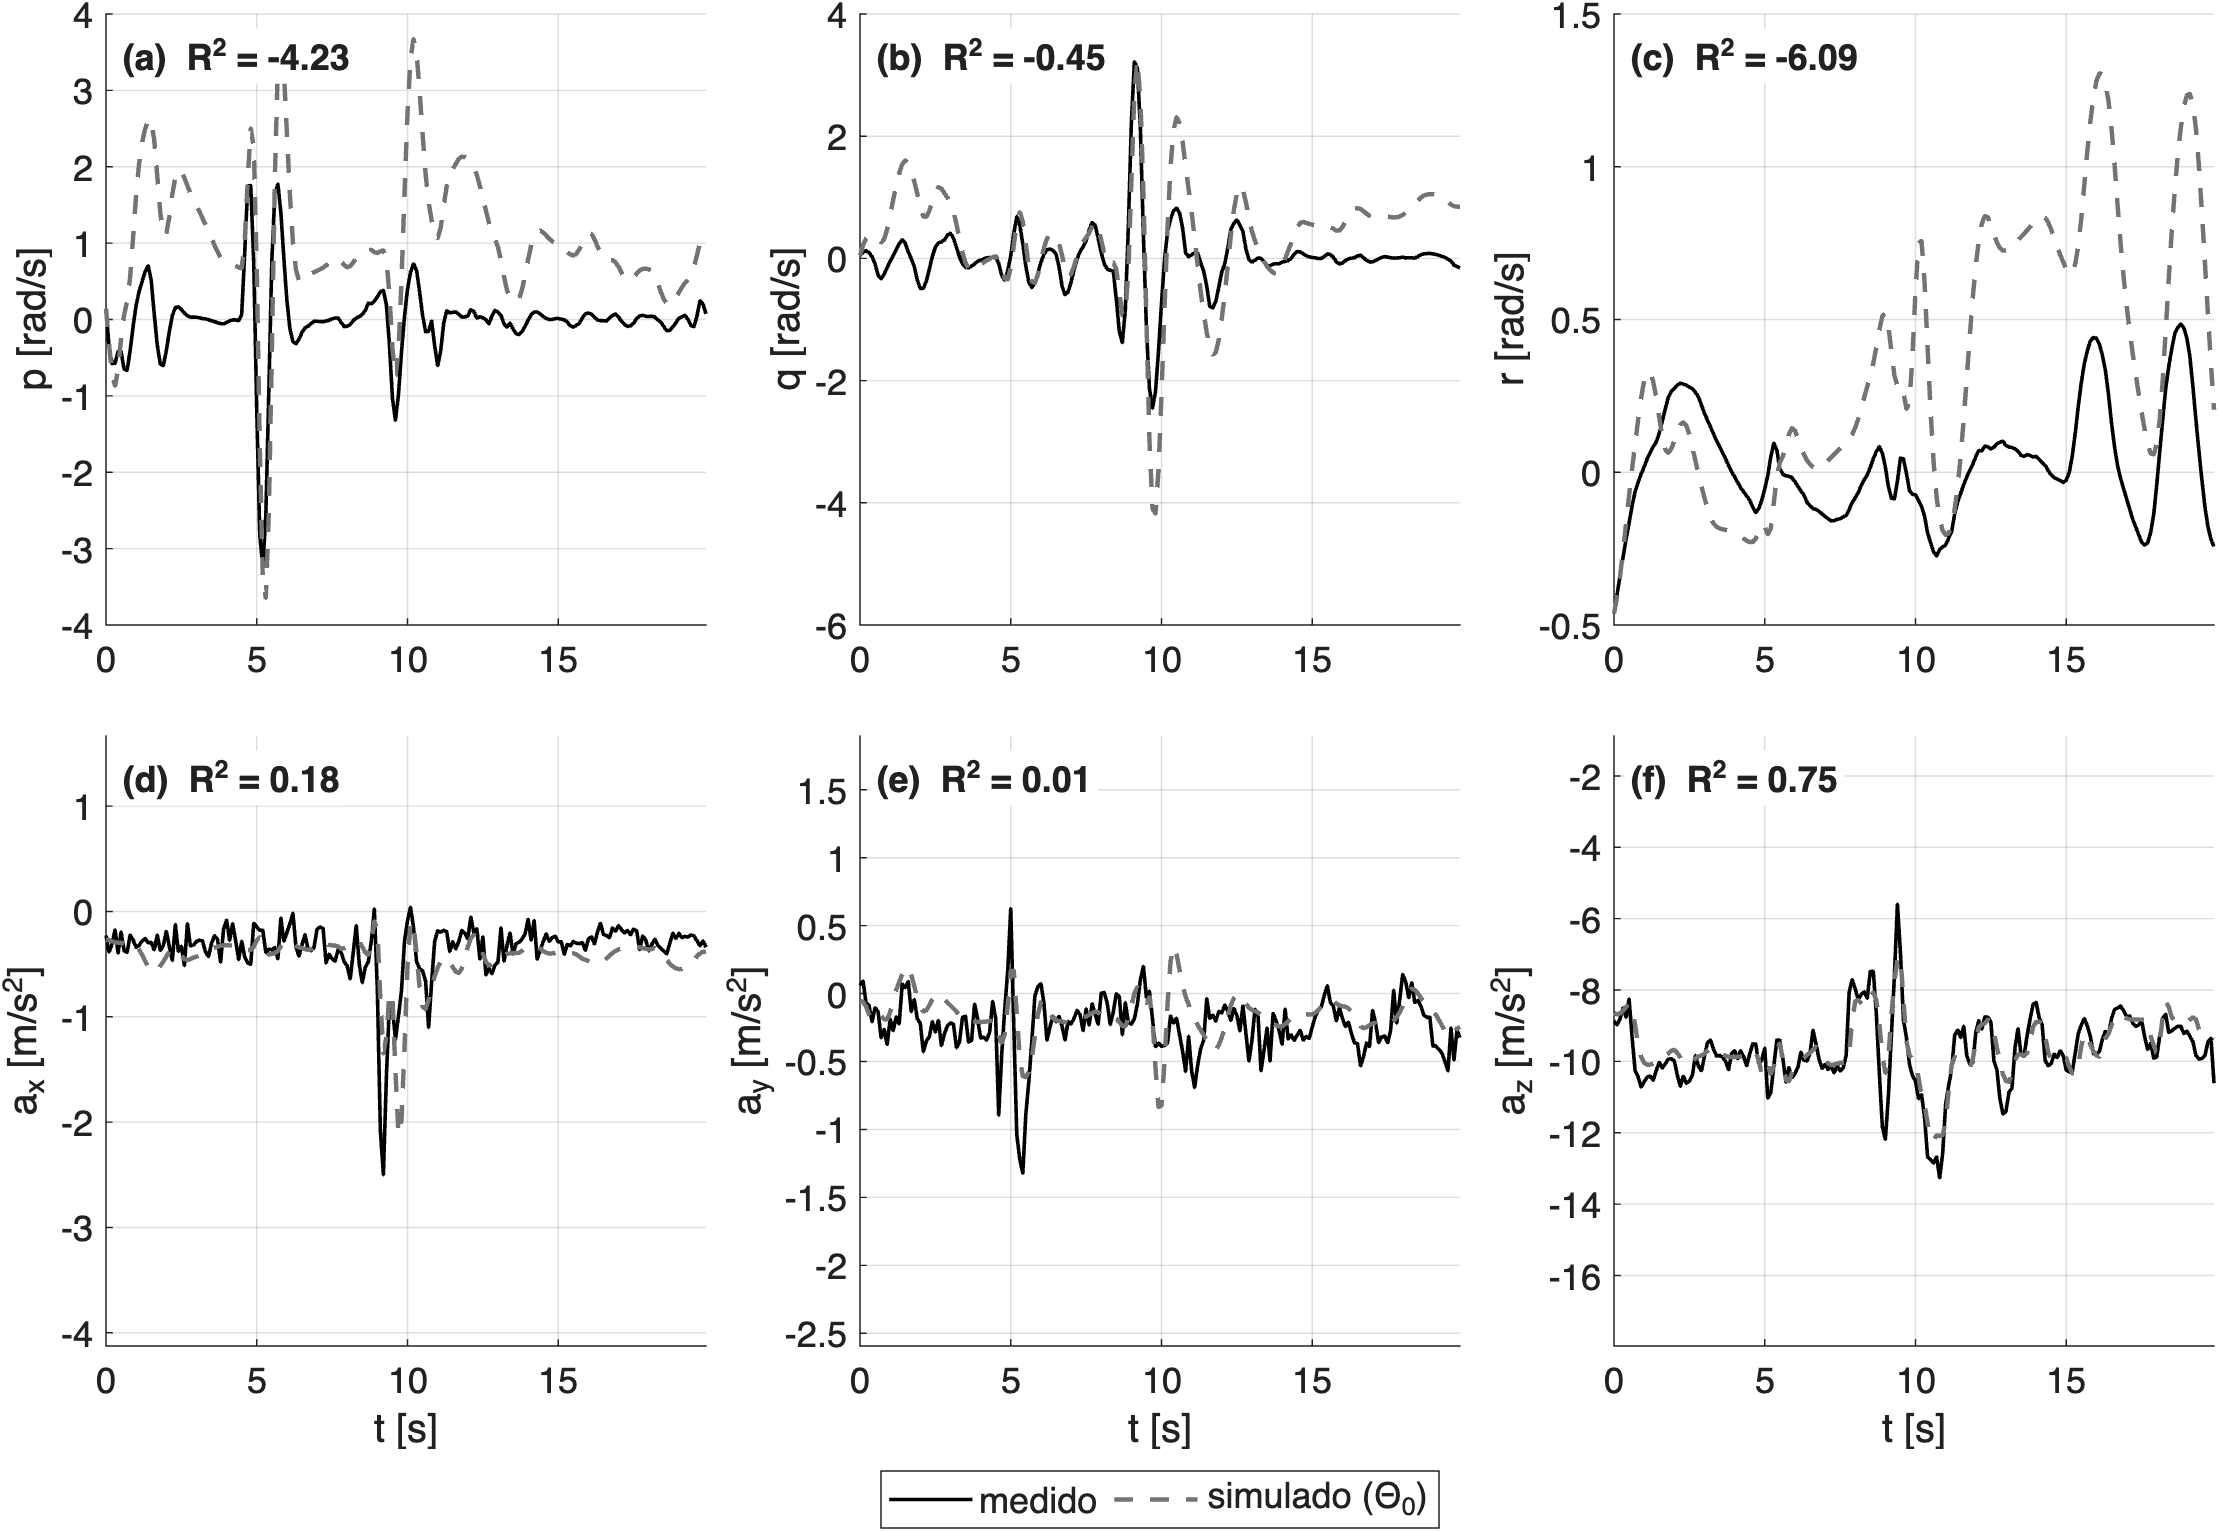
\includegraphics[width=\textwidth]{Cap5/id_sim_p0.png}
    \caption{Resposta simulada do modelo inicial $\Theta_0$ (cinza tracejado) frente às medições (preto contínuo), na janela de validação: (a) $p$, (b) $q$ e (c) $r$, velocidades angulares; (d) $a_x$, (e) $a_y$ e (f) $a_z$, forças específicas. O $R^2$ de cada canal consta no título do painel.}
    \label{fig:sim-p0}
\end{figure}

A Tabela~\ref{tab:params-comp} compara os parâmetros nas três etapas. O EEM fornece um ponto de partida algébrico, porém enviesado, que subestima os coeficientes de empuxo pela atenuação de amplitude da diferenciação numérica das taxas{\color{blue}, e o OEM corrige esse viés, devolvendo cada família de parâmetros a valores fisicamente interpretáveis:
\begin{itemize}
    \item \textbf{coeficientes de empuxo}: sobem para cerca de $1{,}87\times10^{-7}$~N/RPM$^2$, $6\%$ acima da bancada, com os quatro motores a menos de $2\%$ entre si. A correção funciona como uma recalibração da cadeia propulsiva em voo, absorvendo o que o ensaio estático não enxerga, como o estado da bateria sob carga e a interação do escoamento com a estrutura;
    \item \textbf{momentos de inércia}: ficam cerca de $10\%$ acima do modelo tridimensional na rolagem e $14\%$ na arfagem e na guinada. O sentido físico é direto, pois cabeamento, fixações e instrumentação acrescentados ao protótipo não constam do desenho e, distribuídos longe do CG, contribuem com o quadrado do braço para as inércias reais;
    \item \textbf{contratorques}: caem entre $15\%$ e $29\%$, a maior correção relativa de todas, recaindo justamente sobre a medição mais difícil da bancada, um momento pequeno obtido por braço de alavanca. A consequência física é uma autoridade de guinada menor que a prevista, coerente com tudo o que esse canal exibe na sequência;
    \item \textbf{amortecimentos angulares}: superam o valor inicial da teoria de influxo por fatores de $3$ a $11$, quantificando os mecanismos que o cálculo teórico não contempla. O principal candidato são os efeitos aerodinâmicos sobre a asa e a fuselagem induzidos pelo próprio escoamento dos rotores, e não pela velocidade translacional, de modo que atuam mesmo no voo pairado e escapam tanto do cálculo de influxo quanto dos termos aerodinâmicos proporcionais a $V_a$, sem excluir a contribuição de outros fenômenos físicos não modelados para a composição desses valores. O $N_r$ da guinada permanece o menor dos três, coerente com a baixa autoridade desse eixo.
\end{itemize}}

\begin{table}[ht]
    \centering
    \caption{Comparação dos parâmetros e desvio-padrão relativo de Cramér-Rao (CR\%) dos modelos $\Theta_0$, $\Theta_{\text{EEM}}$ e $\Theta_{\text{OEM}}$. Os valores de $c_T$ estão em $10^{-7}$~N/RPM$^2$ e os de $c_M$ em $10^{-9}$~N$\cdot$m/RPM$^2$.}
    \label{tab:params-comp}
    \begin{tabular}{l cc cc cc}
    \toprule
    & \multicolumn{2}{c}{$\Theta_0$} & \multicolumn{2}{c}{$\Theta_{\text{EEM}}$} & \multicolumn{2}{c}{$\Theta_{\text{OEM}}$} \\
    \cmidrule(lr){2-3}\cmidrule(lr){4-5}\cmidrule(lr){6-7}
    Parâmetro & valor & CR\% & valor & CR\% & valor & CR\% \\
    \midrule
    $J_x$    & 0,0432 & 3,8 & 0,0541 & 14,6 & 0,0475 & 2,9 \\
    $J_y$    & 0,0844 & 4,8 & 0,0892 & 13,0 & 0,0963 & 2,6 \\
    $J_z$    & 0,1262 & 5,1 & 0,1433 & 9,9 & 0,1438 & 2,0 \\
    $J_{xz}$ & 0,00157 & 106 & 0,00126 & $6{,}2\times10^{2}$ & 0,00126 & 106 \\
    $c_{T1}$ & 1,76 & 1,5 & 1,09 & 5,3 & 1,86 & 0,8 \\
    $c_{T2}$ & 1,76 & 1,5 & 1,09 & 5,4 & 1,86 & 0,8 \\
    $c_{T3}$ & 1,76 & 1,8 & 1,07 & 6,3 & 1,86 & 0,9 \\
    $c_{T4}$ & 1,76 & 1,7 & 1,09 & 5,8 & 1,89 & 0,8 \\
    $c_{M1}$ & 5,04 & 12,5 & 3,61 & 22,3 & 3,77 & 5,0 \\
    $c_{M2}$ & 5,04 & 12,7 & 3,26 & 25,3 & 3,58 & 5,4 \\
    $c_{M3}$ & 5,04 & 13,2 & 4,52 & 19,0 & 4,28 & 4,7 \\
    $c_{M4}$ & 5,04 & 12,3 & 3,24 & 26,0 & 3,96 & 5,0 \\
    $L_p$    & 0,0513 & 8,8 & 0,1257 & 23,2 & 0,2571 & 6,4 \\
    $M_q$    & 0,1017 & 12,1 & 0,1670 & 25,4 & 0,3492 & 7,8 \\
    $N_r$    & 0,0100 & 19,9 & 0,0838 & 22,9 & 0,1113 & 8,5 \\
    \bottomrule
    \end{tabular}
\end{table}



{\color{blue}A qualidade das estimativas acompanha essa leitura. Pelo limite de Cramér--Rao, todos os parâmetros têm desvio-padrão relativo abaixo de $10\%$, exceto $J_{xz}$, praticamente inobservável. Os mais bem determinados são os coeficientes de empuxo, abaixo de $1\%$, e a faixa mais larga é a da família da guinada, de $2{,}0\%$ a $8{,}5\%$, o canal de pior observabilidade. A matriz de correlação da Figura~\ref{fig:corr-matrix} mostra a origem dessa diferença: fora dela os parâmetros são praticamente descorrelacionados, e as únicas estruturas fortes são o bloco da guinada, com $J_z$ e $N_r$ correlacionados a $+0{,}97$, e os pares da propulsão, com $+0{,}99$ dentro de cada par de $c_T$ e $-0{,}95$ entre os pares dianteiro e traseiro.}

\begin{figure}[H]
    \centering
    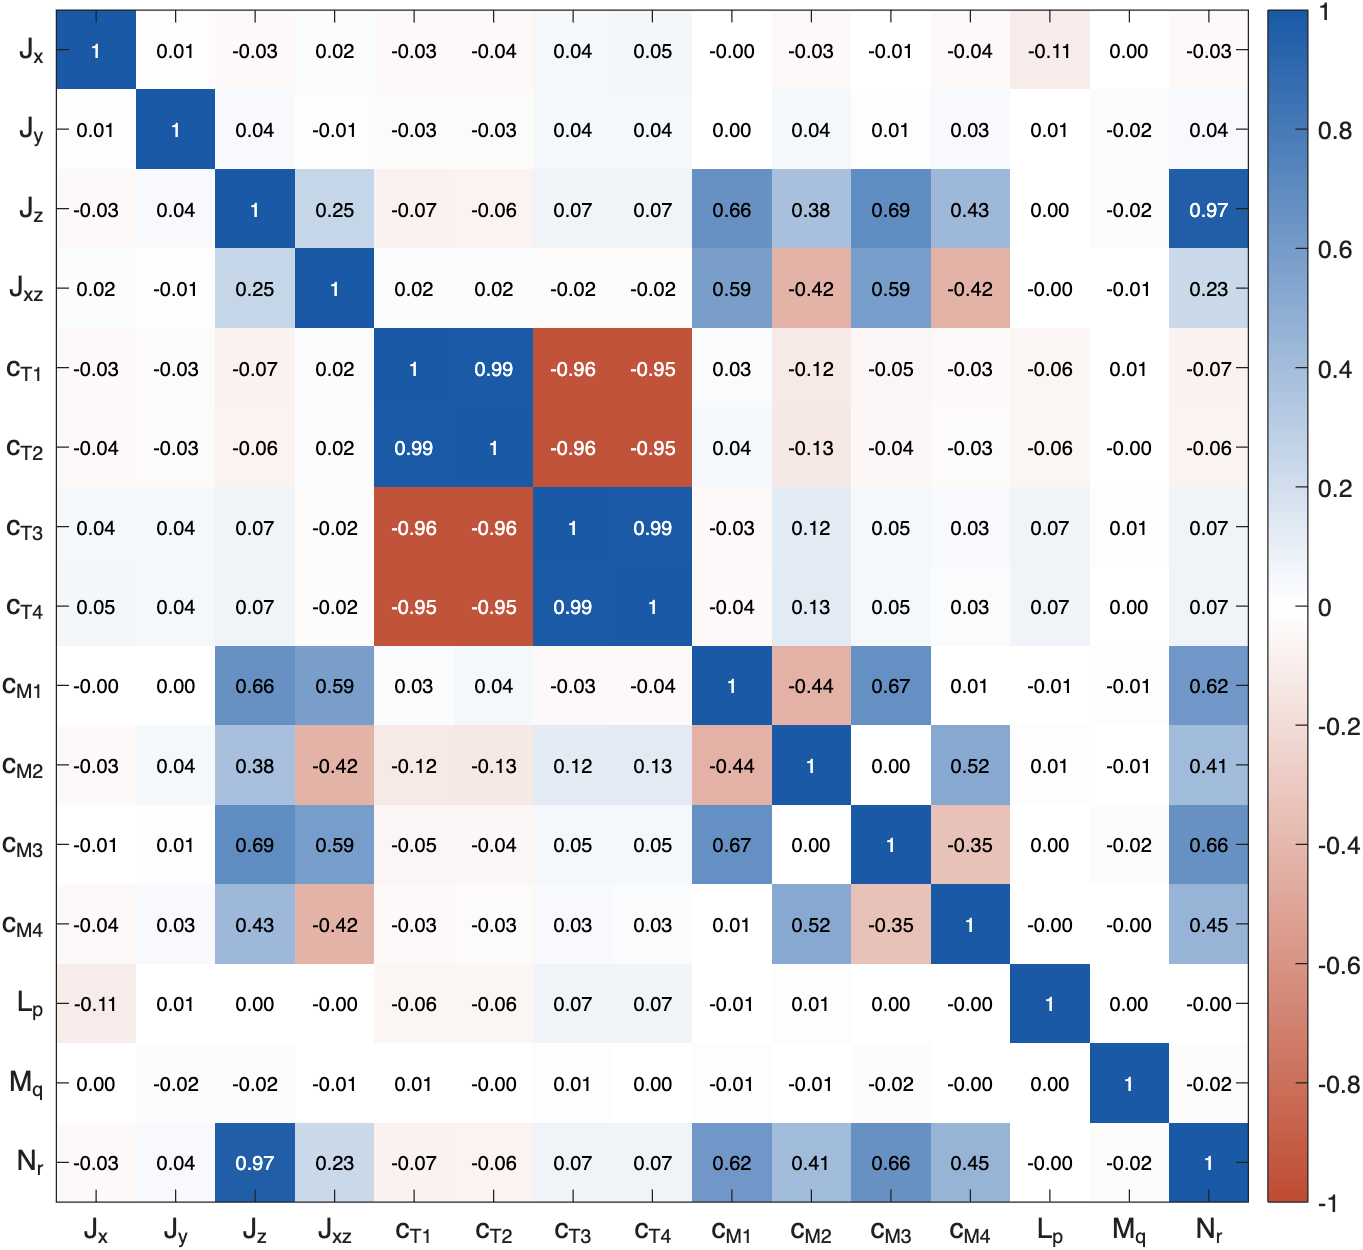
\includegraphics[width=0.88\textwidth]{Cap5/corr_matrix.png}
    \caption{\color{blue}Matriz de correlação das estimativas no ponto identificado, com a observação completa.}
    \label{fig:corr-matrix}
\end{figure} {\color{blue}Nessa condição, $J_z$ deslocou-se até a fronteira da desigualdade triangular de inércia, com $J_z = J_x + J_y$, ao absorver os desvios decorrentes da pouca observabilidade da guinada, e $J_{xz}$ recuou ao limite inferior admitido, comportamento antecipado pela análise de identificabilidade da Seção~\ref{sec:coerencia}.}

{\color{blue}Os estágios progressivos do OEM convergiram para parâmetros próximos, adotando-se o de melhor coeficiente de determinação médio na validação, com $R^2$ de $0{,}70$, $0{,}73$ e $0{,}77$ em $p$, $q$ e $r$. Considerando também as forças específicas, o $R^2$ médio fica em $0{,}57$.}

Por fim, a Figura~\ref{fig:sim-comp} sobrepõe as respostas do modelo inicial $\Theta_0$, da estimativa do EEM e do OEM final às medições{\color{blue}, em simulação contínua de malha aberta sobre o segmento de validação}. A melhora é progressiva: o $\Theta_0$ diverge nas taxas (sobretudo em $p$), o EEM já acompanha a forma geral, e o OEM final adere às medições, {\color{blue}com o $R^2$ de cada canal indicado nos painéis}. No acelerômetro, a resposta de $a_z$ do EEM destaca-se por subestimar o empuxo (reflexo do $c_T$ enviesado), corrigida pelo OEM.

\begin{figure}[!htb]
    \centering
    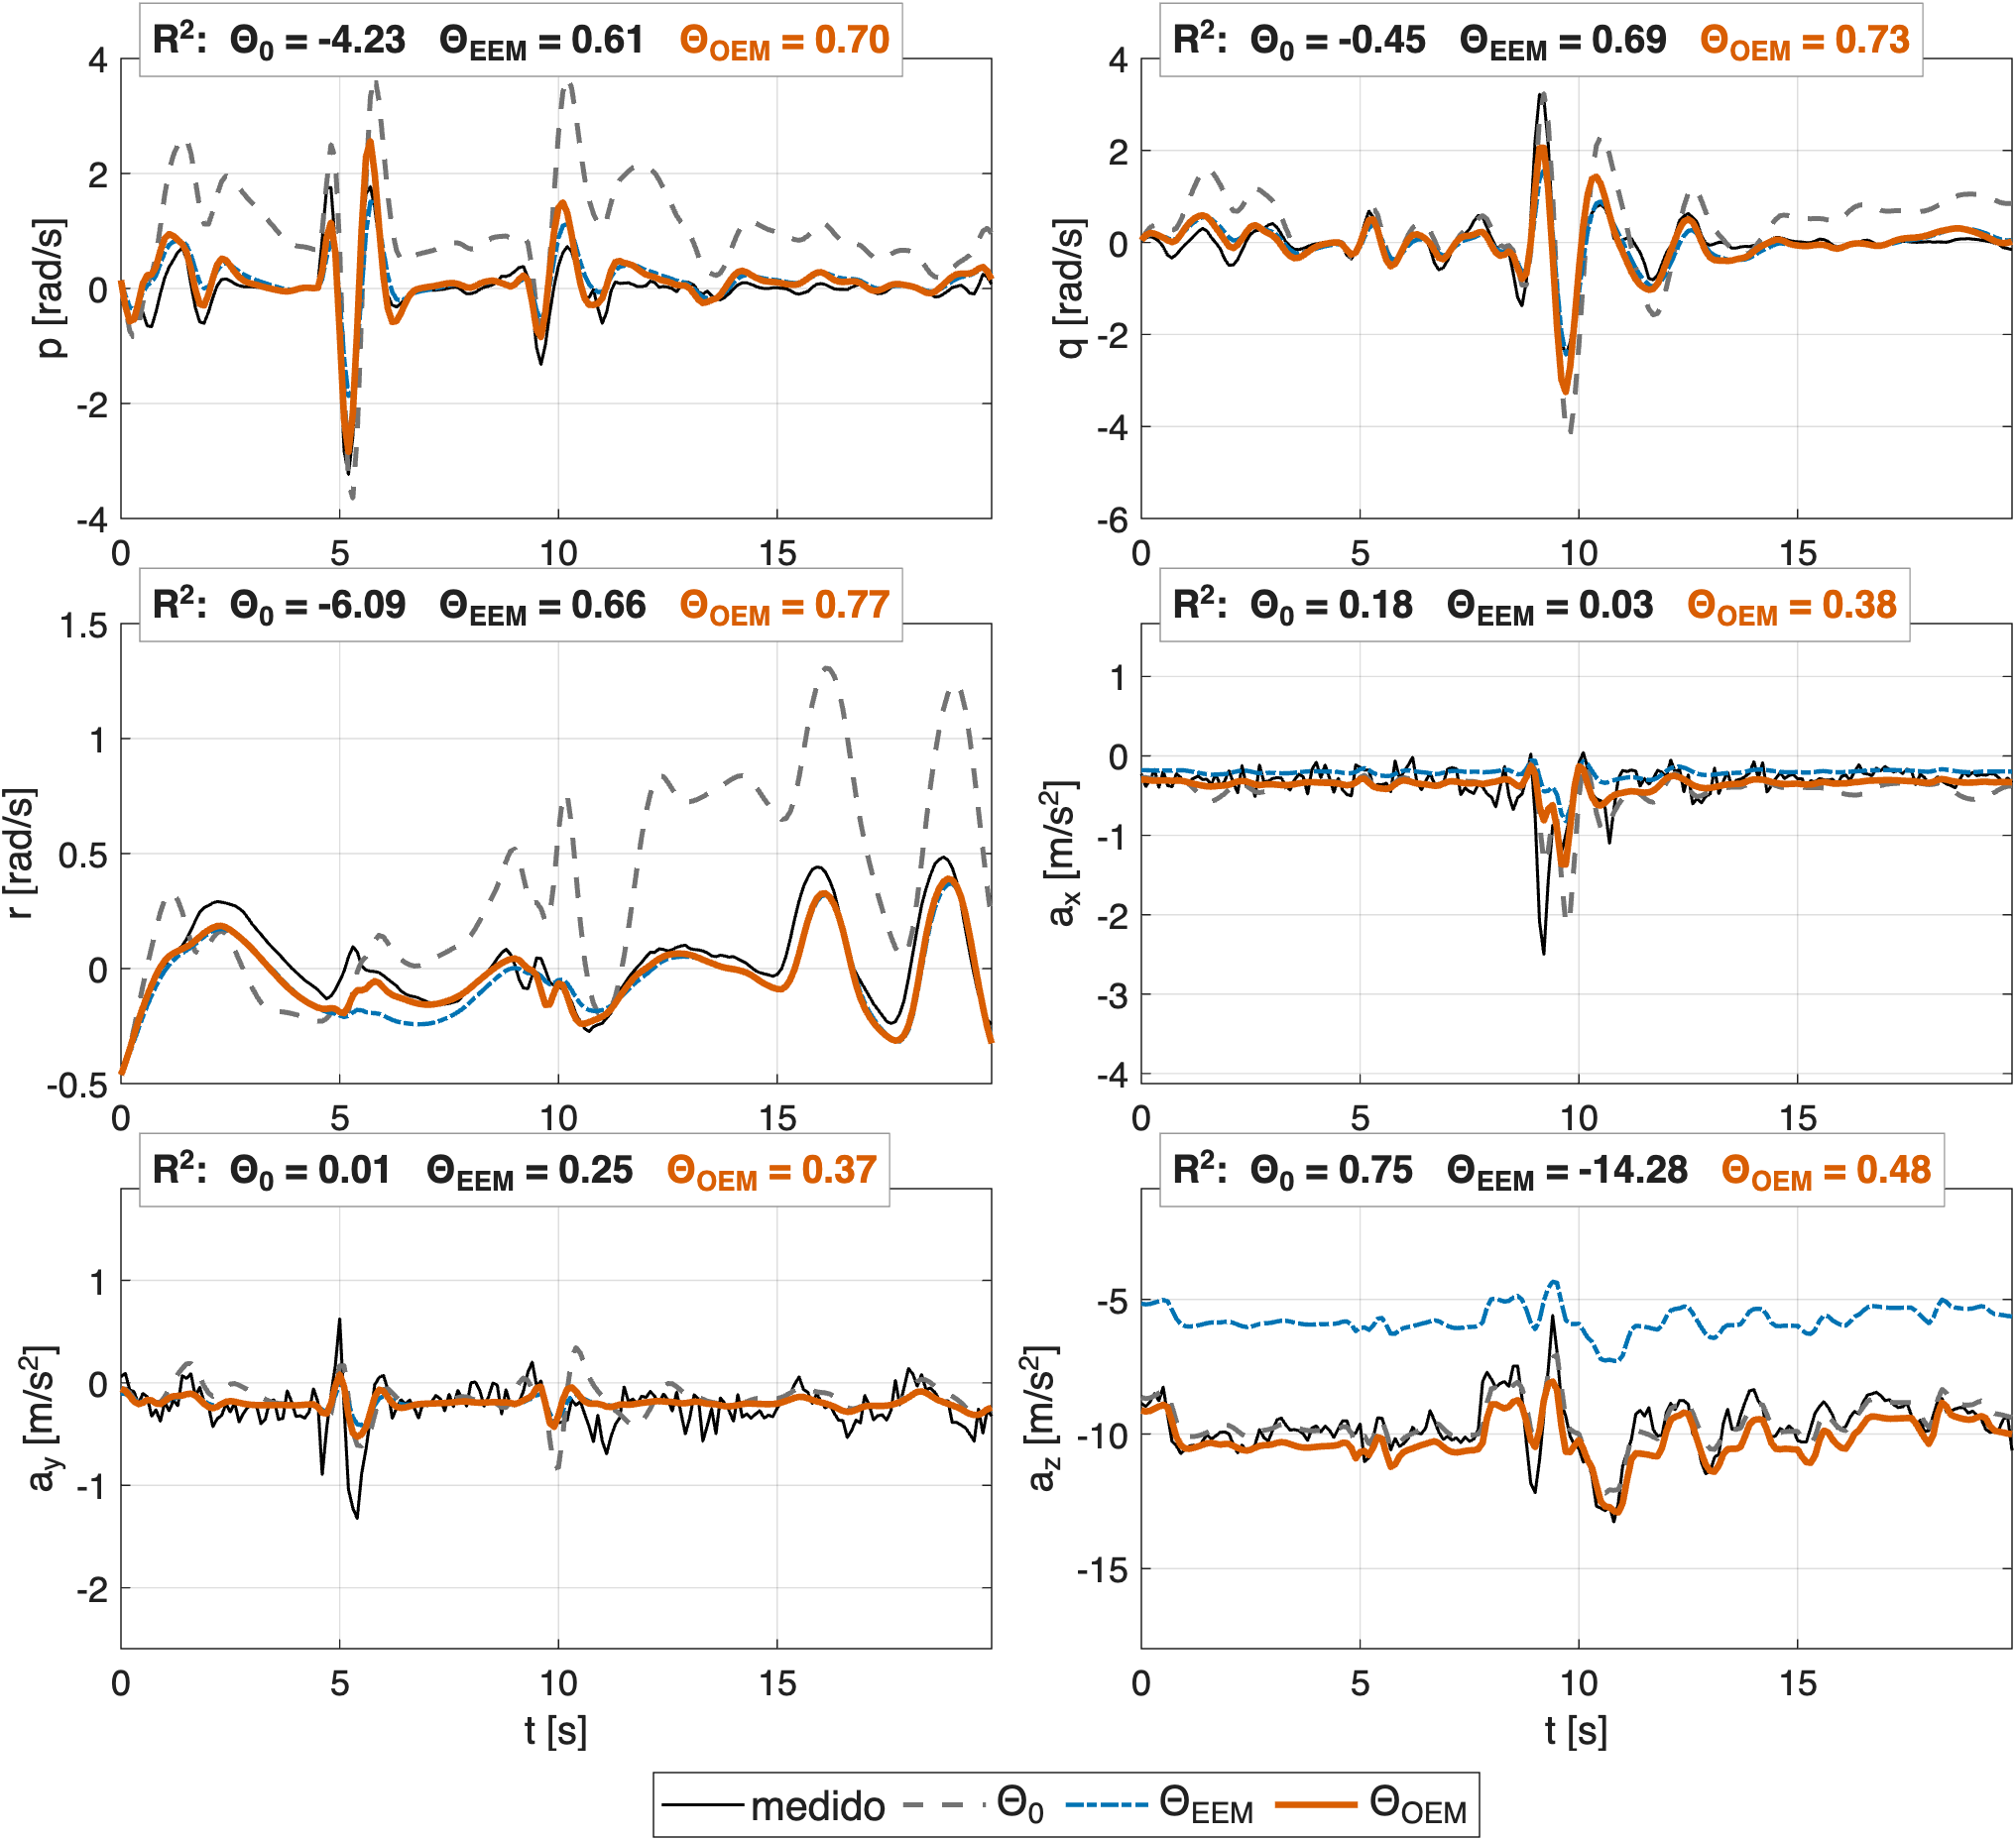
\includegraphics[width=\textwidth,height=0.68\textheight,keepaspectratio]{Cap5/id_comp_all.png}
    \caption{Comparação das respostas de $\Theta_0$, $\Theta_{\text{EEM}}$ e $\Theta_{\text{OEM}}$ frente às medições, nas velocidades angulares e nas forças específicas.}
    \label{fig:sim-comp}
\end{figure}

\section{Validação do Modelo Identificado}

O modelo identificado é validado no segmento de {\color{blue}$610$ a $630$~s}, não utilizado na estimação e rico em movimento composto acoplado nos três eixos{\color{blue}, com avanços e recuos simultâneos e velocidade translacional de até $2{,}8$~m/s, média de $1{,}0$~m/s, dentro do envelope de voo pairado}, simulando a resposta a partir dos comandos PWM registrados e confrontando-a com as medições de $p,q,r$,$a_x$,$a_y$ e $a_z$. A simulação integra o subsistema de taxa com o modelo de motor físico (idêntico ao do estimador). Aplicam-se as métricas definidas no capítulo anterior: o coeficiente de determinação $R^2$ (Equação~\eqref{eq:r2}), o coeficiente de Theil TIC (Equação~\eqref{eq:tic}) e a decomposição de Theil em viés, variância e covariância (Equação~\eqref{eq:theil}). Comparam-se o modelo inicial $\Theta_0$ (Tabela~\ref{tab:val-p0}), sendo a coluna \textit{(at.?)} referente a um indicador se atendeu ao critério, e o resultado final do OEM (Tabela~\ref{tab:val-oem}).

A comparação evidencia o ganho da identificação. O modelo inicial $\Theta_0$ não reproduz a dinâmica de taxa: o $R^2$ é fortemente negativo em $p$, $q$ e $r$ e o TIC é elevado, {\color{blue}com o erro de $p$ dominado pela parcela de viés ($U^b = 0{,}68$). Apenas $a_z$ ($R^2 = 0{,}74$) é razoável, pois $\Theta_0$ já parte do empuxo nominal de bancada.}

\begin{table}[ht]
    \centering
    \caption{Validação do modelo inicial $\Theta_0$}
    \label{tab:val-p0}
    \begin{tabular*}{\textwidth}{@{\extracolsep{\fill}}l cc cc cc cc cc}
    \toprule
     & \multicolumn{2}{c}{$R^2$} & \multicolumn{2}{c}{TIC} & \multicolumn{2}{c}{$U^b$} & \multicolumn{2}{c}{$U^v$} & \multicolumn{2}{c}{$U^c$} \\
    \cmidrule(lr){2-3}\cmidrule(lr){4-5}\cmidrule(lr){6-7}\cmidrule(lr){8-9}\cmidrule(lr){10-11}
    Canal & valor & at.? & valor & at.? & valor & at.? & valor & at.? & valor & at.? \\
    \midrule
    $p$   & $-3{,}83$ & $\times$ & 0,62 & $\times$ & 0,68 & $\times$ & 0,13 & \checkmark & 0,19 & $\times$ \\
    $q$   & $-0{,}38$ & $\times$ & 0,43 & $\times$ & 0,27 & $\times$ & 0,26 & \checkmark & 0,48 & $\times$ \\
    $r$   & $-6{,}54$ & $\times$ & 0,66 & $\times$ & 0,50 & $\times$ & 0,24 & \checkmark & 0,26 & $\times$ \\
    $a_x$ & 0,19 & $\times$ & 0,27 & \checkmark & 0,12 & $\times$ & 0,02 & \checkmark & 0,86 & \checkmark \\
    $a_y$ & 0,04 & $\times$ & 0,40 & $\times$ & 0,14 & $\times$ & 0,09 & \checkmark & 0,77 & \checkmark \\
    $a_z$ & 0,74 & \checkmark & 0,03 & \checkmark & 0,06 & \checkmark & 0,19 & \checkmark & 0,75 & \checkmark \\
    \bottomrule
    \end{tabular*}
\end{table}

\begin{table}[ht]
    \centering
    \caption{Validação do modelo final do OEM.}
    \label{tab:val-oem}
    \begin{tabular*}{\textwidth}{@{\extracolsep{\fill}}l cc cc cc cc cc}
    \toprule
     & \multicolumn{2}{c}{$R^2$} & \multicolumn{2}{c}{TIC} & \multicolumn{2}{c}{$U^b$} & \multicolumn{2}{c}{$U^v$} & \multicolumn{2}{c}{$U^c$} \\
    \cmidrule(lr){2-3}\cmidrule(lr){4-5}\cmidrule(lr){6-7}\cmidrule(lr){8-9}\cmidrule(lr){10-11}
    Canal & valor & at.? & valor & at.? & valor & at.? & valor & at.? & valor & at.? \\
    \midrule
    $p$   & 0,70 & \checkmark & 0,27 & \checkmark & 0,25 & $\times$ & 0,00 & \checkmark & 0,75 & \checkmark \\
    $q$   & 0,73 & \checkmark & 0,26 & \checkmark & 0,01 & \checkmark & 0,00 & \checkmark & 0,99 & \checkmark \\
    $r$   & 0,77 & \checkmark & 0,25 & \checkmark & 0,42 & $\times$ & 0,06 & \checkmark & 0,52 & \checkmark \\
    $a_x$ & 0,38 & $\times$ & 0,26 & \checkmark & 0,01 & \checkmark & 0,41 & $\times$ & 0,58 & \checkmark \\
    $a_y$ & 0,37 & $\times$ & 0,33 & $\times$ & 0,04 & \checkmark & 0,71 & $\times$ & 0,25 & $\times$ \\
    $a_z$ & 0,48 & $\times$ & 0,04 & \checkmark & 0,40 & $\times$ & 0,09 & \checkmark & 0,51 & \checkmark \\
    \bottomrule
    \end{tabular*}
\end{table}

{\color{blue}O modelo do OEM, por outro lado, reproduz bem as taxas: $R^2$ de $0{,}70$, $0{,}73$ e $0{,}77$ em $p$, $q$ e $r$, com TIC de $0{,}25$ a $0{,}27$, dentro do limite de bom ajuste, e o erro residual dominado pela parcela de covariância em $p$ e $q$ ($U^c$ de $0{,}75$ e $0{,}99$), indicando resíduo essencialmente aleatório, sem viés sistemático nem erro de amplitude. Na guinada, que apresenta o maior $R^2$, persiste um viés residual ($U^b = 0{,}42$), coerente com a menor observabilidade do canal. O acelerômetro é reproduzido de forma moderada ($R^2$ de $0{,}37$ a $0{,}48$): em $a_z$ persiste um viés ($U^b = 0{,}40$) associado ao patamar de empuxo no voo pairado, e em $a_x$ e $a_y$ a parcela de variância torna-se relevante ($0{,}41$ e $0{,}71$), refletindo os limites do modelo de sensor para as forças específicas laterais.}

{\color{blue}
\section[{\color{blue}Influência dos Efeitos Aerodinâmicos da Estrutura}]{Influência dos Efeitos Aerodinâmicos da Estrutura}
\label{sec:aero-influencia}

Para quantificar o que a simplificação de quadrirrotor absorve nos parâmetros estimados, conduziram-se duas identificações idênticas, diferindo apenas pela presença dos termos aerodinâmicos da estrutura da Seção~\ref{sec:aero-estrutura}, que entram com coeficientes fixos, escalados pela velocidade estimada de bordo, sem disputar conteúdo dos dados com os parâmetros livres{\color{blue}, com os amortecimentos resultantes das duas identificações reunidos na Tabela~\ref{tab:aero-absorcao}}.
\begin{table}[ht]
\centering
\caption{\color{blue}Amortecimentos identificados com e sem os termos aerodinâmicos da estrutura proporcionais à velocidade translacional.}
\label{tab:aero-absorcao}
\color{blue}
\begin{tabular}{l c c c}
\toprule
Parâmetro [N$\cdot$m$\cdot$s] & com termos & sem termos & variação \\
\midrule
$L_p$ & 0,2571 & 0,2633 & $+2{,}4\%$ \\
$M_q$ & 0,3492 & 0,3718 & $+6{,}5\%$ \\
$N_r$ & 0,1113 & 0,1149 & $+3{,}3\%$ \\
\bottomrule
\end{tabular}
\end{table}



O efeito de absorção existe, porém é pequeno: sem os termos aerodinâmicos os amortecimentos identificados aumentam 2\% em $L_p$, 6\% em $M_q$ e 3\% em $N_r$, sempre abaixo do limite de Cramér-Rao, e na validação em doze janelas fora do treino o coeficiente de determinação médio e o TIC variam no máximo 0,038 e 0,009. A Figura~\ref{fig:val_aero_comp} mostra respostas praticamente indistinguíveis, com a maior separação na guinada, o eixo de maior contribuição relativa da asa, no qual os termos aerodinâmicos elevam o $R^2$ de $0{,}73$ para $0{,}81$. Uma explicação possível é que o giro do corpo em torno do próprio eixo vertical impõe às semiasas uma velocidade translacional local, proporcional ao braço e à taxa $r$, de modo que a asa enxerga escoamento mesmo sem avanço da aeronave, tornando a guinada o eixo mais sensível à presença desses termos.



\begin{figure}[!htb]
    \centering
    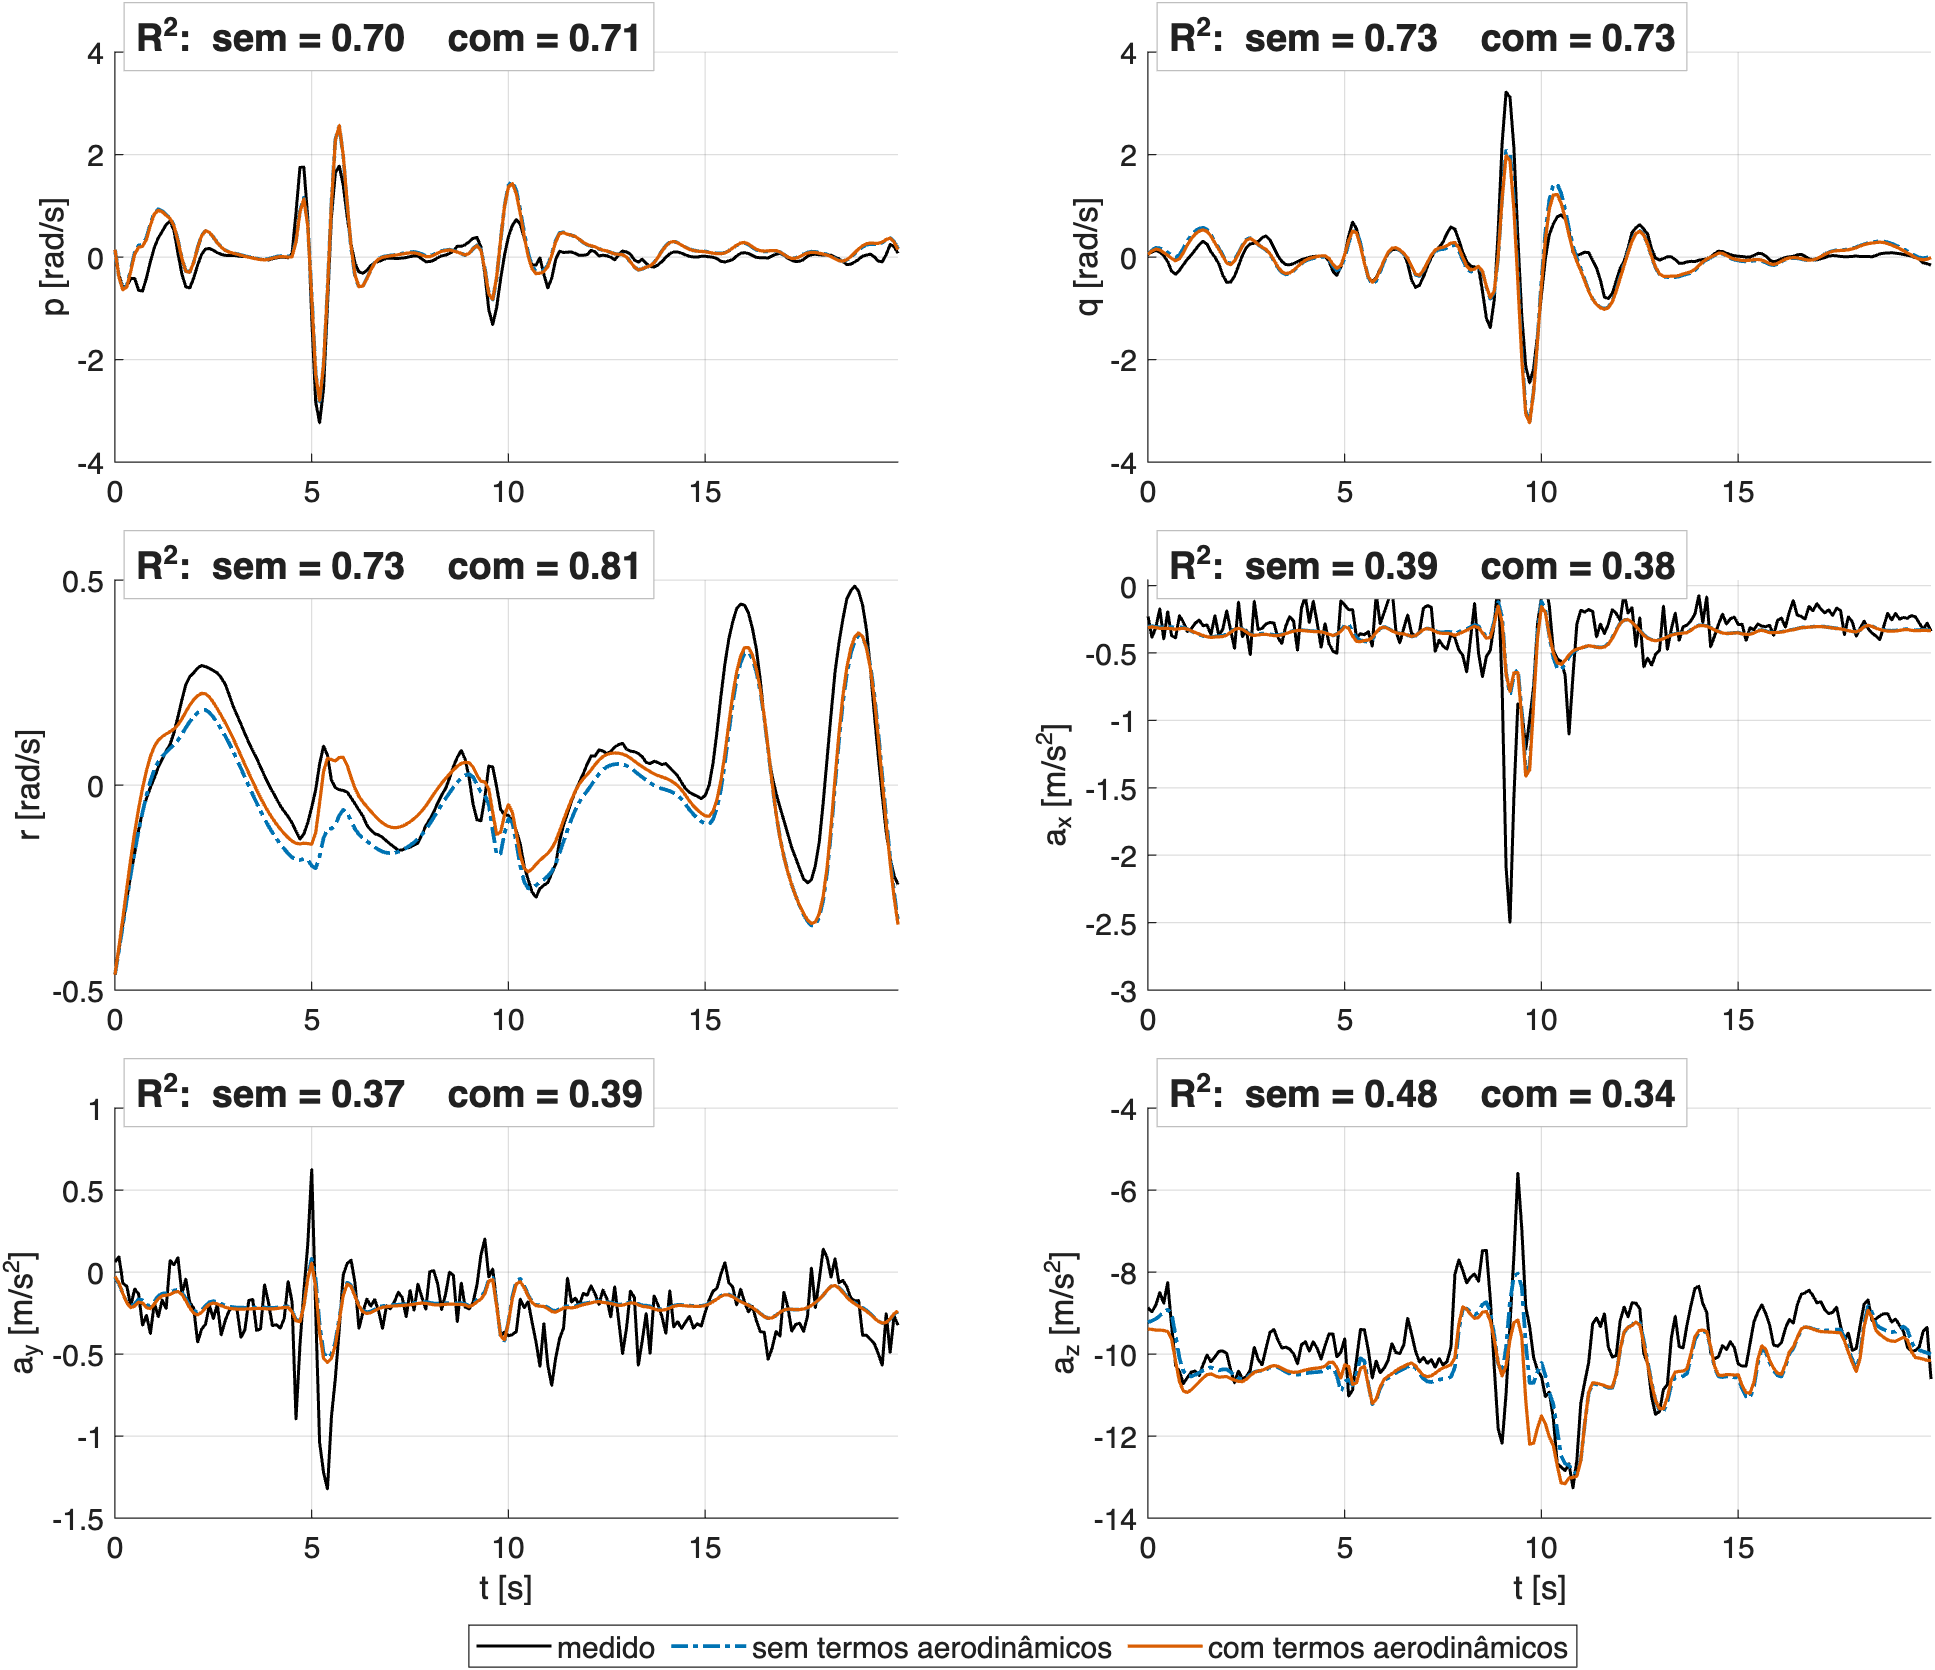
\includegraphics[width=\textwidth,height=0.62\textheight,keepaspectratio]{Cap5/val_aero_comp.png}
    \caption{{\color{blue}Validação em malha aberta no segmento de 610 a 630~s com os modelos identificados sem e com os termos aerodinâmicos da estrutura, sobrepostos às medições, com o $R^2$ de cada canal indicado nos painéis.}}
    \label{fig:val_aero_comp}
\end{figure}

Esses resultados delimitam a validade da simplificação. No envelope ensaiado, com velocidade translacional inferior a $3$~m/s, tratar a aeronave como quadrirrotor convencional introduz nos parâmetros um desvio menor que a incerteza com que são determinados, e acima dele o modelo com os termos da estrutura degrada-se de forma previsível, enquanto o simplificado perde validade sem qualquer indicação interna. Nas velocidades intermediárias as duas parcelas multiplicam os mesmos estados e tornam-se colineares nos dados, de modo que nenhuma identificação naquele regime atribui o esforço medido a uma ou a outra fonte. Caracterizar cada efeito no extremo em que é observável é, portanto, o delineamento experimental bem posto para essa classe de aeronave, e entrega os dois extremos validados a partir dos quais a transição poderá ser modelada.
}

\section{Definição da Arquitetura em Cascata}

O controle de voo do VTOL em modo multirrotor é organizado em uma arquitetura em cascata, composta por malhas de realimentação aninhadas, cada uma responsável por uma grandeza e operando em uma escala de tempo distinta \cite{Hu2024, Beard2012, Idrissi2022, Mohsan2022}. As malhas externas, mais lentas, regulam posição e velocidade; as internas, mais rápidas, regulam atitude e velocidade angular. Essa separação por escalas de tempo permite projetar cada malha de forma independente. A interna por ser muito mais rápida, é vista pela externa como aproximadamente instantânea, o que confere modularidade ao projeto \cite{Hu2024}.

\begin{figure}[ht]
    \centering
    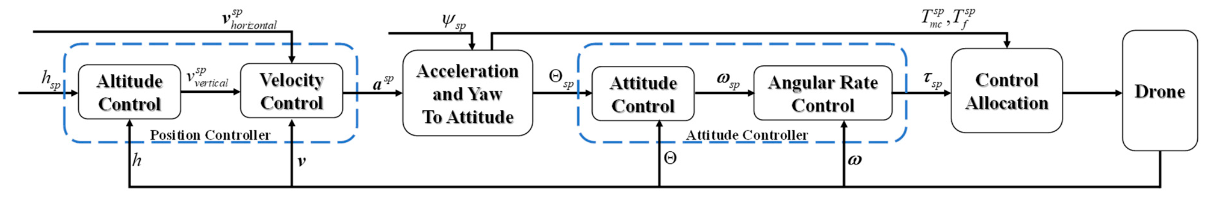
\includegraphics[width=1\textwidth]{Cap4/control.png}
    \caption{Arquitetura PID cascata \cite{Hu2024}.}
    \label{fig:cascata}
\end{figure}

A Figura~\ref{fig:cascata} apresenta a estrutura completa, da referência de comando até os atuadores. O fluxo, da malha mais externa para a mais interna, é:
\begin{itemize}
    \item \textbf{Controlador de posição} (controle de altitude + controle de velocidade): a partir da altitude de referência $h_{sp}$ e da velocidade horizontal de referência $\mathbf{v}^{sp}_{hor}$, realimentado pela altitude $h$ e pela velocidade $\mathbf{v}$ medidas, gera uma \emph{aceleração de referência} $\mathbf{a}^{sp}$;
    \item \textbf{Conversão de aceleração e guinada em atitude}: combina a aceleração de referência $\mathbf{a}^{sp}$ com a guinada de referência $\psi_{sp}$ para produzir a \emph{atitude de referência} $\Theta_{sp}$;
    \item \textbf{Controlador de atitude} (controle de atitude + controle de velocidade angular): a partir de $\Theta_{sp}$ gera a velocidade angular de referência $\boldsymbol{\omega}_{sp}$ e, desta, o \emph{momento de referência} $\boldsymbol{\tau}_{sp}$, realimentado pela atitude $\Theta$ e pela velocidade angular $\boldsymbol{\omega}$ medidas;
    \item \textbf{Alocação de controle}: converte o momento de referência $\boldsymbol{\tau}_{sp}$ e o empuxo total nos comandos individuais dos atuadores, fechando a cadeia até o drone, conforme a matriz de alocação deduzida no Capítulo~2.
\end{itemize}

A malha mais interna de velocidade angular corresponde justamente à dinâmica identificada nas seções anteriores, onde o modelo de taxa estimado por OEM é a planta sobre a qual essa malha é projetada, de modo que a qualidade da identificação reflete-se diretamente no desempenho do controle de atitude. Modelos de planta mais sofisticados, que capturam efeitos aerodinâmicos por abordagens híbridas combinando princípios físicos e aprendizado de máquina \cite{Bauersfeld2021}, são possíveis, porém o modelo de corpo rígido identificado mostra-se suficiente para o controle em torno do voo pairado. Cada malha é implementada por um controlador PID com saturação, projetado nas seções seguintes.

A arquitetura da Figura~\ref{fig:cascata} serve como referência conceitual geral. Neste trabalho adotou-se uma realização simplificada e desacoplada dela, suficiente para o controle em torno do voo pairado e coerente com o modelo identificado. As simplificações são:
\begin{itemize}
    \item cada eixo é tratado como uma malha SISO independente, o que se justifica pelo acoplamento cruzado desprezível do modelo linear, em que o momento de guinada gera sobre a rolagem apenas $\Gamma_4\approx0{,}27$ contra $\Gamma_3\approx21{,}3$ na própria diagonal (cerca de $1\%$), já que o produto de inércia $J_{xz}$ é ínfimo, fato que a simulação confirma adiante;
    \item a atitude é controlada por um PD em cada eixo, proporcional ao erro de ângulo e derivativo na velocidade angular medida, de modo que a malha de velocidade angular fica embutida no termo derivativo, sem uma referência $\boldsymbol{\omega}_{sp}$ explícita;
    \item da velocidade horizontal controla-se apenas a componente de avanço, com a rolagem regulada em zero, e o comando de atitude resulta diretamente do erro de velocidade, sem o estágio intermediário de aceleração de referência $\mathbf{a}^{sp}$;
    \item a altitude é regulada diretamente pelo empuxo total, com realimentação direta do peso.
\end{itemize}

\section{Projeto de Controladores PID}

Cada malha da cascata foi projetada de forma independente por alocação de polos sobre o modelo de taxa identificado por OEM, linearizado em torno do voo pairado conforme o Apêndice~\ref{ap:linearizacao}. Os coeficientes que entram no projeto são, portanto, lidos diretamente das matrizes $A$ e $B$ desse modelo linear, de modo que a qualidade da identificação propaga-se para os ganhos obtidos. O procedimento é direto. Para cada malha escolhe-se uma frequência natural $\omega_n$ e um fator de amortecimento $\zeta$, que traduzem a especificação de desempenho desejada, ou seja, a rapidez de resposta e o sobressinal aceitável. Em seguida igualam-se os coeficientes do polinômio característico de malha fechada aos do polinômio de segunda ordem de referência $s^2+2\zeta\omega_n s+\omega_n^2$, e os ganhos resultam dessa igualdade.

As malhas internas de atitude foram projetadas mais rápidas que as externas de velocidade e altitude, com separação de banda de cerca de quatro vezes. Assim a malha interna responde de modo praticamente instantâneo para a malha externa, e ambas podem ser ajustadas sem interação significativa.

\subsection{Malhas de atitude}

A dinâmica de atitude usada no projeto vem da linearização, em torno do voo pairado, das equações rotacionais identificadas nas seções anteriores. Tomando a rolagem como exemplo, a Equação~\eqref{eq:p_dot} fornece: 

$\dot p=\Gamma_1 pq-\Gamma_2 qr+\Gamma_3\tau_x+\Gamma_4\tau_z-c_p\,p$. 
Perto do hover as velocidades angulares são pequenas, de modo que os produtos giroscópicos ($pq$, $qr$) e o acoplamento de guinada ($\Gamma_4\tau_z$) tornam-se desprezíveis, restando $\dot p\approx -c_p\,p+\Gamma_3\,\tau_x$. Como, nessa condição, a cinemática de Euler reduz-se a $\dot\phi=p$, segue que $\ddot\phi\approx-c_p\,\dot\phi+\Gamma_3\,\tau_x$. Cada eixo de atitude assume, assim, a forma de segunda ordem
\begin{equation}
\ddot{\alpha}=-a\,\dot{\alpha}+b\,\tau,
\label{eq:att-2ord}
\end{equation}
em que $\alpha$ é o ângulo, $a$ o arrasto angular e $b$ a efetividade de controle. O arrasto $a$ é o coeficiente $c_p$, $c_q$ ou $c_r$ identificado, e a efetividade $b$ é o termo de inércia correspondente ($\Gamma_3$ na rolagem, $1/J_y$ na arfagem e $\Gamma_8$ na guinada), ambos lidos diretamente das matrizes do modelo linear na forma $a=-A_{ii}$ e $b=B_{ij}$.

A lei é um PD na forma $\tau=K_p(\alpha_c-\alpha)-K_d\,\dot{\alpha}$, cujo polinômio de malha fechada é $s^2+(a+bK_d)\,s+bK_p$. Igualando à forma de referência obtêm-se os ganhos
\begin{equation}
K_p=\frac{\omega_n^2}{b}, \qquad K_d=\frac{2\zeta\omega_n-a}{b}.
\label{eq:gain-att}
\end{equation}
A Tabela~\ref{tab:gain-att} apresenta, por eixo, os coeficientes $a$ e $b$ do modelo, a especificação $(\omega_n,\zeta)$ e os ganhos obtidos.

\begin{table}[ht]
\centering
\caption{Coeficientes do modelo, especificação e ganhos das malhas de atitude.}
\label{tab:gain-att}
\begin{tabular}{l c c c c c c}
\toprule
Eixo & $a$ [s$^{-1}$] & $b$ [(kg$\cdot$m$^2)^{-1}$] & $\omega_n$ [rad/s] & $\zeta$ & $K_p$ & $K_d$ \\
\midrule
Rolagem ($\phi$)   & 6,85 & 21,33 & 6,0 & 0,8 & 1,69 & 0,13 \\
Arfagem ($\theta$) & 4,68 & 10,71 & 6,0 & 0,8 & 3,36 & 0,46 \\
Guinada ($\psi$)   & 0,81 &  7,93 & 2,5 & 0,8 & 0,79 & 0,40 \\
\bottomrule
\end{tabular}
\end{table}

\subsection{Malha de velocidade de avanço}

Com a atitude interna rápida, a velocidade longitudinal segue $\dot{u}\approx-g\,\theta$. Comanda-se o ângulo de arfagem por um PI na forma $\theta_c=-\left(K_p\,e_u+K_i\!\int e_u\,dt\right)/g$, o que leva à dinâmica $s^2+K_p\,s+K_i$ e, portanto, aos ganhos
\begin{equation}
K_p=2\zeta\omega_n, \qquad K_i=\omega_n^2.
\label{eq:gain-u}
\end{equation}
Nesta malha a especificação fixa diretamente os ganhos, sem depender da planta, como mostra a Tabela~\ref{tab:gain-u}.

\begin{table}[ht]
\centering
\caption{Valores de projeto e ganhos da malha de velocidade de avanço.}
\label{tab:gain-u}
\begin{tabular}{l c}
\toprule
Grandeza & Valor \\
\midrule
$g$ [m/s$^2$]      & 9,81 \\
$\omega_n$ [rad/s] & 1,5  \\
$\zeta$            & 0,9  \\
$K_p$              & 2,70 \\
$K_i$              & 2,25 \\
\bottomrule
\end{tabular}
\end{table}

\subsection{Malha de altitude}

A altitude é um duplo integrador acionado pelo empuxo, $\ddot{h}=\delta T/m$, controlado por um PID com realimentação direta do peso $m g$. Os ganhos resultam em
\begin{equation}
K_p=m\,\omega_n^2, \qquad K_d=2\,m\,\zeta\,\omega_n.
\label{eq:gain-h}
\end{equation}
O termo integral é mantido nulo, uma vez que a realimentação direta de $mg$ já cancela o erro de regime. A Tabela~\ref{tab:gain-h} reúne os valores empregados.

\begin{table}[ht]
\centering
\caption{Valores de projeto e ganhos da malha de altitude.}
\label{tab:gain-h}
\begin{tabular}{l c}
\toprule
Grandeza & Valor \\
\midrule
$m$ [kg]           & 1,993 \\
$\omega_n$ [rad/s] & 2,0  \\
$\zeta$            & 0,9  \\
$K_p$              & 7,97 \\
$K_d$              & 7,18 \\
\bottomrule
\end{tabular}
\end{table}

Por fim, dois limites garantem a operação segura do controlador. O ângulo de arfagem comandado pela malha de velocidade é saturado em vinte graus, e os integradores de velocidade e de altitude são limitados, com anti-windup condicional que congela a integração enquanto o comando permanece saturado, conforme a Tabela~\ref{tab:ctrl-lim}.

\begin{table}[ht]
\centering
\caption{Limites de saturação e anti-windup do controlador.}
\label{tab:ctrl-lim}
\begin{tabular}{l c}
\toprule
Limite & Valor \\
\midrule
Ângulo de arfagem comandado ($\theta_c$) & $\pm 20^\circ$ \\
Integrador de velocidade & $\pm 5{,}0$ \\
Integrador de altitude   & $\pm 5{,}0$ \\
\bottomrule
\end{tabular}
\end{table}

\section{Simulação no Modelo Linear}

Para avaliar a arquitetura projetada, a malha fechada foi simulada sobre o mesmo modelo linearizado em torno do voo pairado empregado no projeto dos ganhos, cujos coeficientes vêm da identificação por OEM apresentada nas seções anteriores. O estado é integrado por Runge--Kutta de quarta ordem com passo de $10$\,ms, partindo do voo pairado nivelado, e o controlador em cascata recebe uma sequência de degraus desacoplados que exercita as três malhas externas: altitude de $0$ para $2$\,m em $t=1$\,s, velocidade longitudinal de $0$ para $3$\,m/s em $t=8$\,s e guinada de $0$ para $30^\circ$ em $t=16$\,s.

\subsection{Saturação dos atuadores}

Diferentemente de uma simulação puramente linear, em que a planta receberia o comando $[\,T,\ \tau_x,\ \tau_y,\ \tau_z\,]$ de forma irrestrita, aqui o limite físico dos motores é imposto dentro da malha. A cada passo o comando do controlador é alocado nos quatro empuxos individuais pela inversa da matriz de alocação~$B$ deduzida no Capítulo~2,
\begin{equation}
\mathbf{T}_{mot}=B^{-1}\,[\,T,\ \tau_x,\ \tau_y,\ \tau_z\,]^{\mathsf{T}} ,
\label{eq:aloc-inv}
\end{equation}
e cada empuxo é convertido no respectivo sinal de PWM pela inversão do modelo de motor da Equação~\eqref{eq:motor-thrust}. O PWM é então saturado na faixa física $[\,1200,\ 2000\,]\ \mu$s, em que o piso de $1200\ \mu$s corresponde à marcha lenta do rotor armado, abaixo da qual o motor não mantém rotação, e reconvertido em empuxo efetivo; aplicando novamente~$B$, recompõe-se o esforço $[\,T,\ \tau_x,\ \tau_y,\ \tau_z\,]_{ef}$ que a planta de fato recebe. Assim a resposta de malha fechada reflete o que os atuadores conseguem entregar, e não o comando ideal. Esse limite soma-se às proteções já internas ao controlador, a saturação do ângulo de arfagem comandado em $\pm 20^\circ$ e o anti-\textit{windup} condicional dos integradores, da Tabela~\ref{tab:ctrl-lim}.

\subsection{Resultados}

A Figura~\ref{fig:sim-control-linear} apresenta a resposta completa. As três malhas externas seguem suas referências com erro de regime praticamente nulo: a altitude estabiliza em $2$\,m com sobressinal de $0{,}1\%$, a velocidade de avanço em $3$\,m/s com $14{,}9\%$ e a guinada em $30^\circ$ com $1{,}5\%$. O sobressinal mais alto na velocidade decorre da saturação do ângulo de arfagem comandado, que atinge o limite de $\pm 20^\circ$ durante a aceleração (visível no painel de atitude, em que $\theta_c$ ultrapassa $\theta$). As malhas internas de atitude permanecem bem amortecidas, com rolagem máxima de apenas $1{,}27^\circ$, evidenciando o desacoplamento entre os eixos.

O painel inferior mostra o PWM dos quatro motores. O empuxo total exigido alcança $30{,}2$\,N no degrau de altitude, próximo do teto de $4\times 7{,}65 = 30{,}6$\,N do conjunto, o que leva os quatro motores ao limite superior de $2000\ \mu$s. Na manobra de guinada o binário diferencial necessário empurra um par de motores ao limite superior e o outro ao inferior ($1200\ \mu$s, a marcha lenta), o único instante em que se observa saturação inferior. No total, o comando demandado excursiona de $594$ a $2248\ \mu$s,fora da faixa física, mas a saturação atua em apenas $1{,}9\%$ dos instantes, concentrados nesses dois transitórios mais agressivos. Mesmo nesses trechos a malha permanece estável e o seguimento é preservado, com um pequeno afundamento de altitude durante a guinada decorrente do acoplamento entre o binário de guinada e o empuxo. O resultado confirma que os ganhos projetados produzem uma resposta rápida e bem amortecida e que a autoridade de controle dos motores é suficiente para as manobras consideradas, esgotando-se apenas nos picos de exigência simultânea.

\begin{figure}[ht]
    \centering
    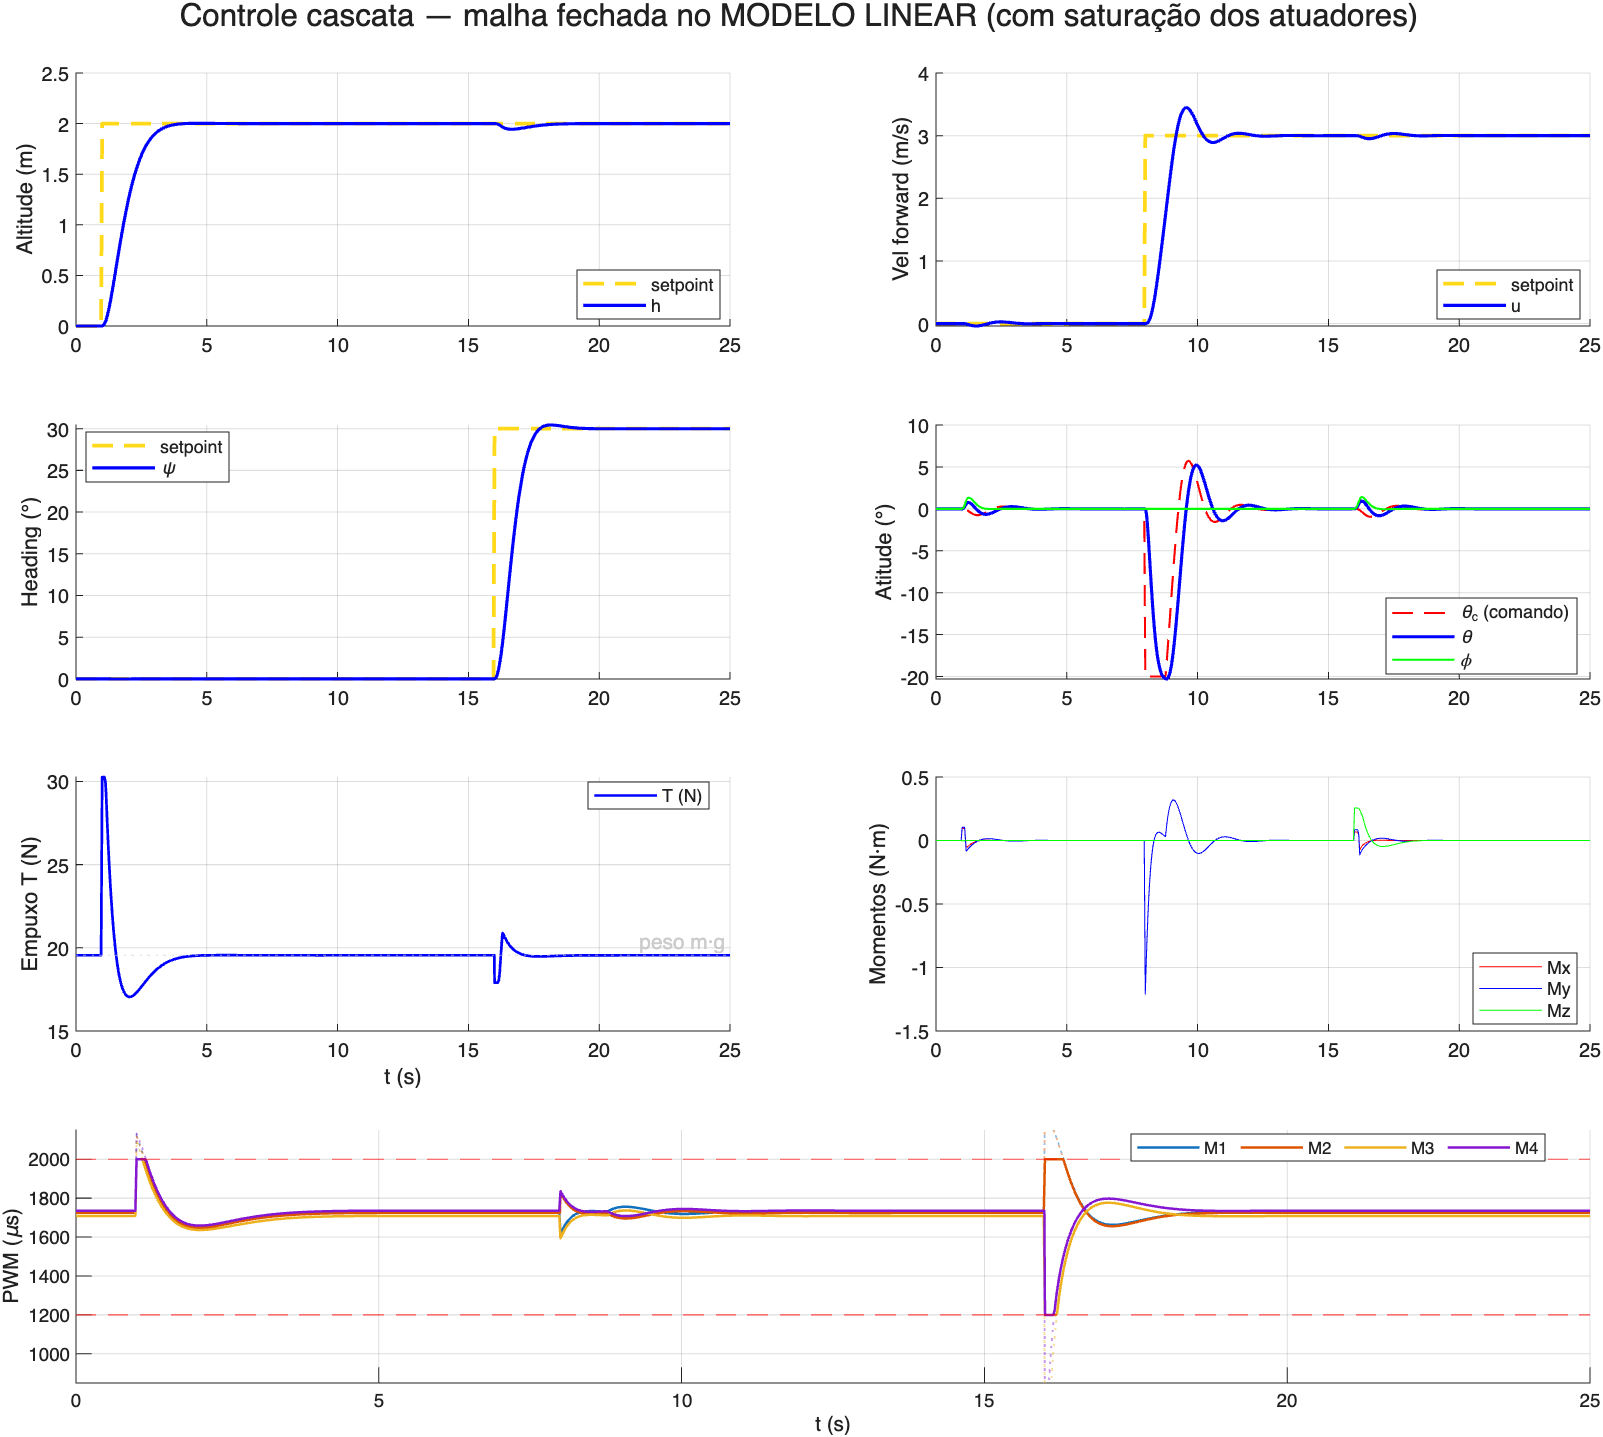
\includegraphics[width=1\textwidth]{Cap4/sim_control_linear.png}
    \caption{Resposta de malha fechada do controle em cascata sobre o modelo linear, com saturação dos atuadores.}
    \label{fig:sim-control-linear}
\end{figure}

\section{Comparação do Controle no Modelo Linear e Não Linear}
\label{sec:ctrl-cmp}

A arquitetura de controle projetada nas seções anteriores sobre o modelo linearizado é agora confrontada com a planta não linear de corpo rígido do Capítulo~\ref{chap:modelagem}, para mapear até onde a linearização em torno do voo pairado permanece válida. Em ambos os casos aplica-se a mesma lei de controle em cascata e a mesma cadeia de atuação, alocação nos quatro motores, saturação de PWM em $[\,1200,\ 2000\,]\ \mu$s e curva real do motor, de modo que a única diferença entre as respostas é a planta: linear, $\dot{\mathbf{x}}=A\mathbf{x}+B(\mathbf{u}-\mathbf{u}_0)$, ou não linear, integrando as equações completas de corpo rígido e a posição inercial.

Duas não linearidades, desprezadas na linearização de voo pairado, ganham peso à medida que a manobra se afasta dessa condição:
\begin{itemize}
    \item o \textbf{acoplamento giroscópico} $-\Gamma_2\,q\,r$ da Equação~\eqref{eq:p_dot}, que gera um torque de rolagem sempre que as taxas de arfagem ($q$) e de guinada ($r$) ocorrem simultaneamente, termo que o modelo linear, com os eixos desacoplados, ignora (prevê $\phi\equiv 0$);
    \item a \textbf{inclinação do vetor de empuxo}: ao arfar um ângulo $\theta$, a componente vertical do empuxo cai com $\cos\theta$, fazendo a altitude afundar; o modelo linear, que trata o empuxo como puramente vertical, não captura esse acoplamento.
\end{itemize}

Para evidenciar a transição, simula-se uma manobra combinada, um pulso de velocidade de avanço (que gera arfagem $q$) sobreposto a um giro {\color{blue}de guinada mantido até $15$~s} (que sustenta $r$), em três níveis de agressividade, escalados por um único fator que cresce de $S_1$ a $S_3$. {\color{blue}O giro é encerrado antes do fim da janela de $30$~s justamente para expor as duas fases da resposta: o comportamento sob o acoplamento sustentado e a convergência quando ele cessa.} A Tabela~\ref{tab:ctrl-cmp} resume os desvios máximos entre as duas plantas, e as Figuras~\ref{fig:ctrl-s1} a~\ref{fig:ctrl-s3} mostram, para cada cenário, as saídas (altitude, velocidade, guinada e rolagem) com seus \emph{setpoints} e as entradas de controle (momentos e PWM). Cabe uma observação sobre a guinada: como a sua referência nesses cenários é uma rampa e a malha é um PD sobre um sistema do tipo 1, o erro de rastreamento converge para um valor constante e não nulo, proporcional à taxa de giro, comportamento esperado da teoria clássica. Esse erro é idêntico nas duas plantas, não decorre do modelo, e não afeta a comparação, cujo objeto são os desvios entre as plantas linear e não linear. Para referências em degrau, como as do projeto, o erro de regime da guinada é nulo, conforme a Seção~\ref{sec:sim-linear}.

\begin{table}[ht]
\centering
\caption{Desvio máximo entre as plantas linear e não linear sob o mesmo controlador, nos três níveis de manobra.}
\label{tab:ctrl-cmp}
\begin{tabular}{l c c c c c}
\toprule
Cenário & $u_{amp}$ [m/s] & spin [°/s] & máx$|\Delta h|$ [m] & máx$|\Delta u|$ [m/s] & máx$|\Delta\phi|$ [°] \\
\midrule
$S_1$ (suave) & 1,2 & 12 & 0,15 & 0,10 & 0,9  \\
$S_2$ (média) & 2,8 & 28 & 0,56 & {\color{blue}1,24} & {\color{blue}2,7}  \\
$S_3$ (forte) & 4,5 & 45 & {\color{blue}1,58} & {\color{blue}9,1} & {\color{blue}11,3} \\
\bottomrule
\end{tabular}
\end{table}

No cenário suave $S_1$ (Figura~\ref{fig:ctrl-s1}), as duas plantas coincidem em regime, mas diferem no transitório. A velocidade de avanço e a guinada se sobrepõem, enquanto a altitude e a rolagem revelam dinâmicas que o modelo linear não representa: a planta não linear afunda $0{,}15$\,m durante o pulso de velocidade, pela perda de sustentação vertical ao inclinar, e desenvolve rolagem de até $0{,}9^\circ$, pelo acoplamento giroscópico entre arfagem e guinada, ao passo que o modelo linear mantém ambas rigorosamente constantes. Esses desvios, contudo, são pequenos em amplitude e desaparecem no regime permanente. Dentro do envelope de voo pairado, portanto, o modelo linear reproduz a planta real a menos de efeitos de acoplamento de segunda ordem, o que valida o controlador projetado sobre ele para manobras suaves.

\begin{figure}[H]
    \centering
    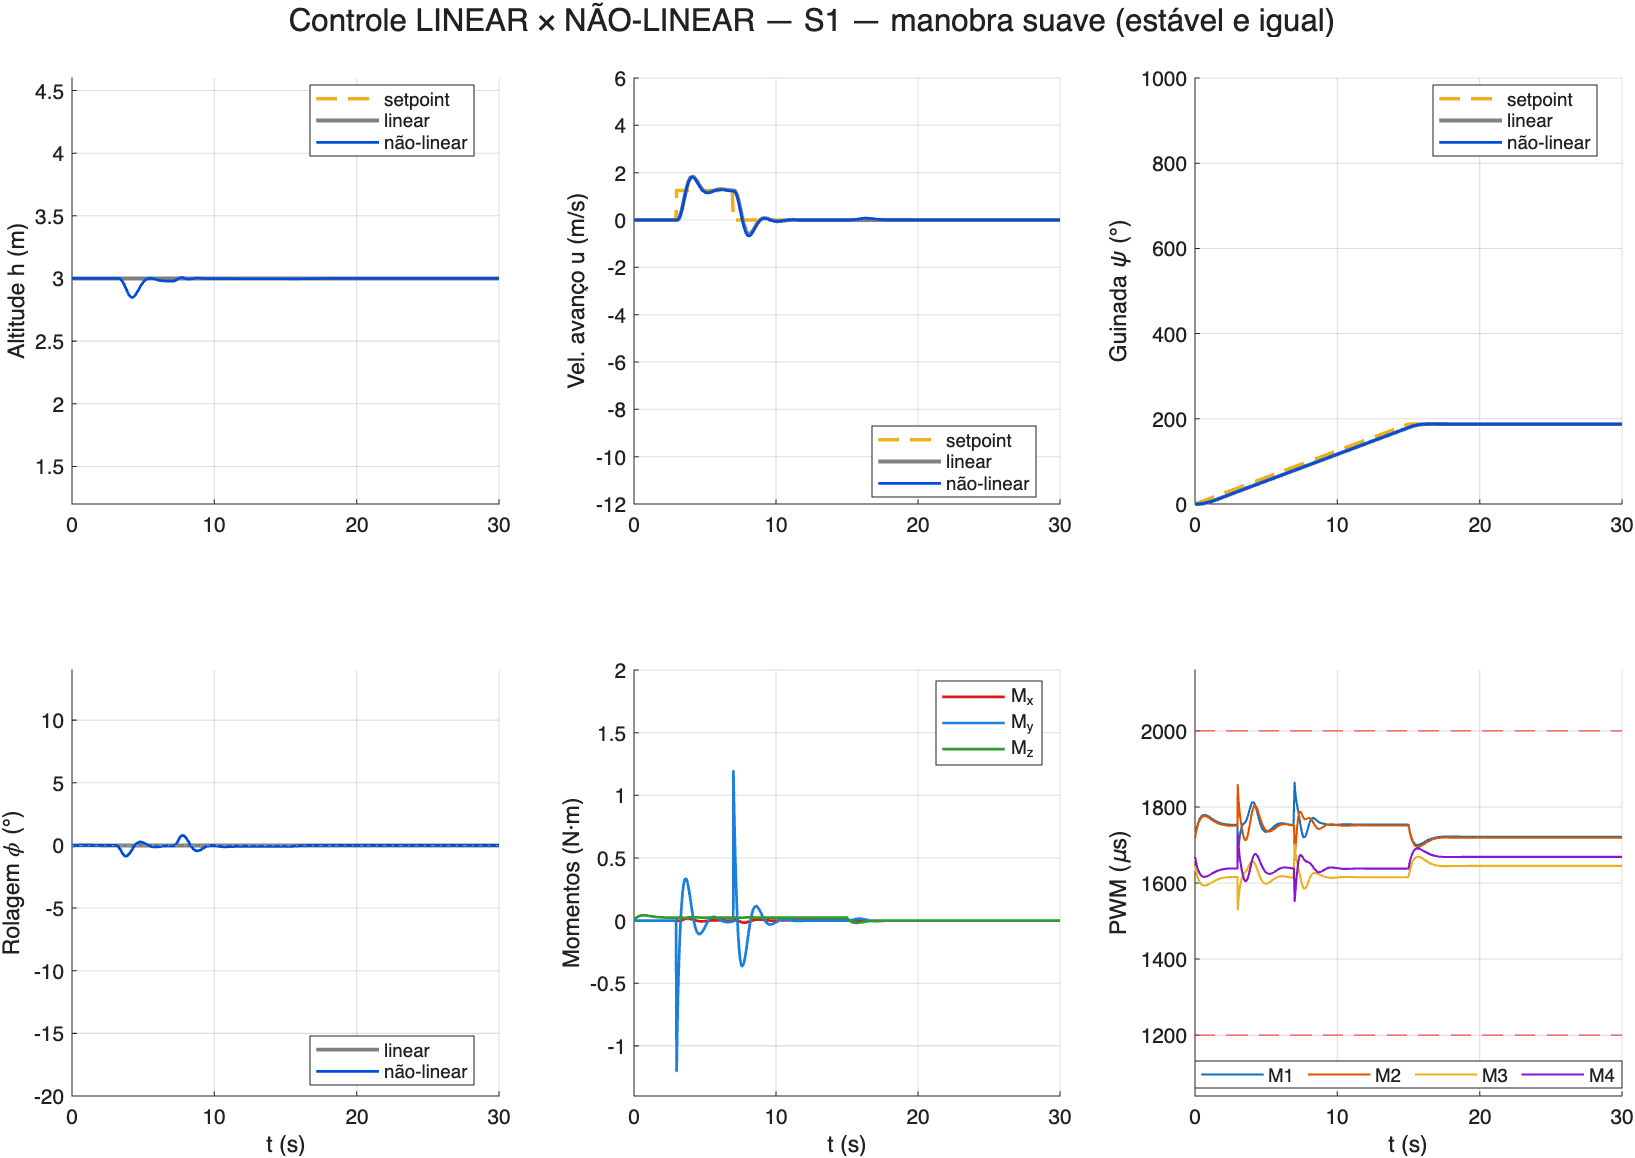
\includegraphics[width=\textwidth]{Cap5/sim_ctrl_s1_igual.png}
    \caption{Cenário $S_1$ (manobra suave): controlador no modelo linear (cinza) e não linear (azul) com os \emph{setpoints} (tracejado). As respostas coincidem em regime, com pequenos desvios transitórios de altitude e rolagem no não linear.}
    \label{fig:ctrl-s1}
\end{figure}

No cenário médio $S_2$ (Figura~\ref{fig:ctrl-s2}), a divergência torna-se visível: a altitude do modelo não linear afunda até cerca de $2{,}5$\,m durante o avanço ($\Delta h = 0{,}56$\,m), enquanto a linear se mantém nivelada, e a rolagem do não linear oscila {\color{blue}cerca de $\pm 3^\circ$} em resposta ao termo $-\Gamma_2\,q\,r$, ausente no linear. {\color{blue}Cabe notar que, na planta não linear, altitude e rolagem não se acomodam enquanto o giro dura: o acoplamento com a arfagem atua como uma excitação persistente, e não como um transitório que se extingue, de modo que ambas mantêm desvio sustentado de pequena amplitude e a rolagem conserva um resíduo de poucos graus. Quando o giro cessa, em $15$~s, essa excitação desaparece e as duas variáveis convergem às referências no restante da janela. A resposta é, portanto, limitada e estável, mas só volta a ser bem comportada, como no cenário suave, após o fim do giro.} A velocidade de avanço e a guinada continuam a seguir as referências nas duas plantas.

\begin{figure}[H]
    \centering
    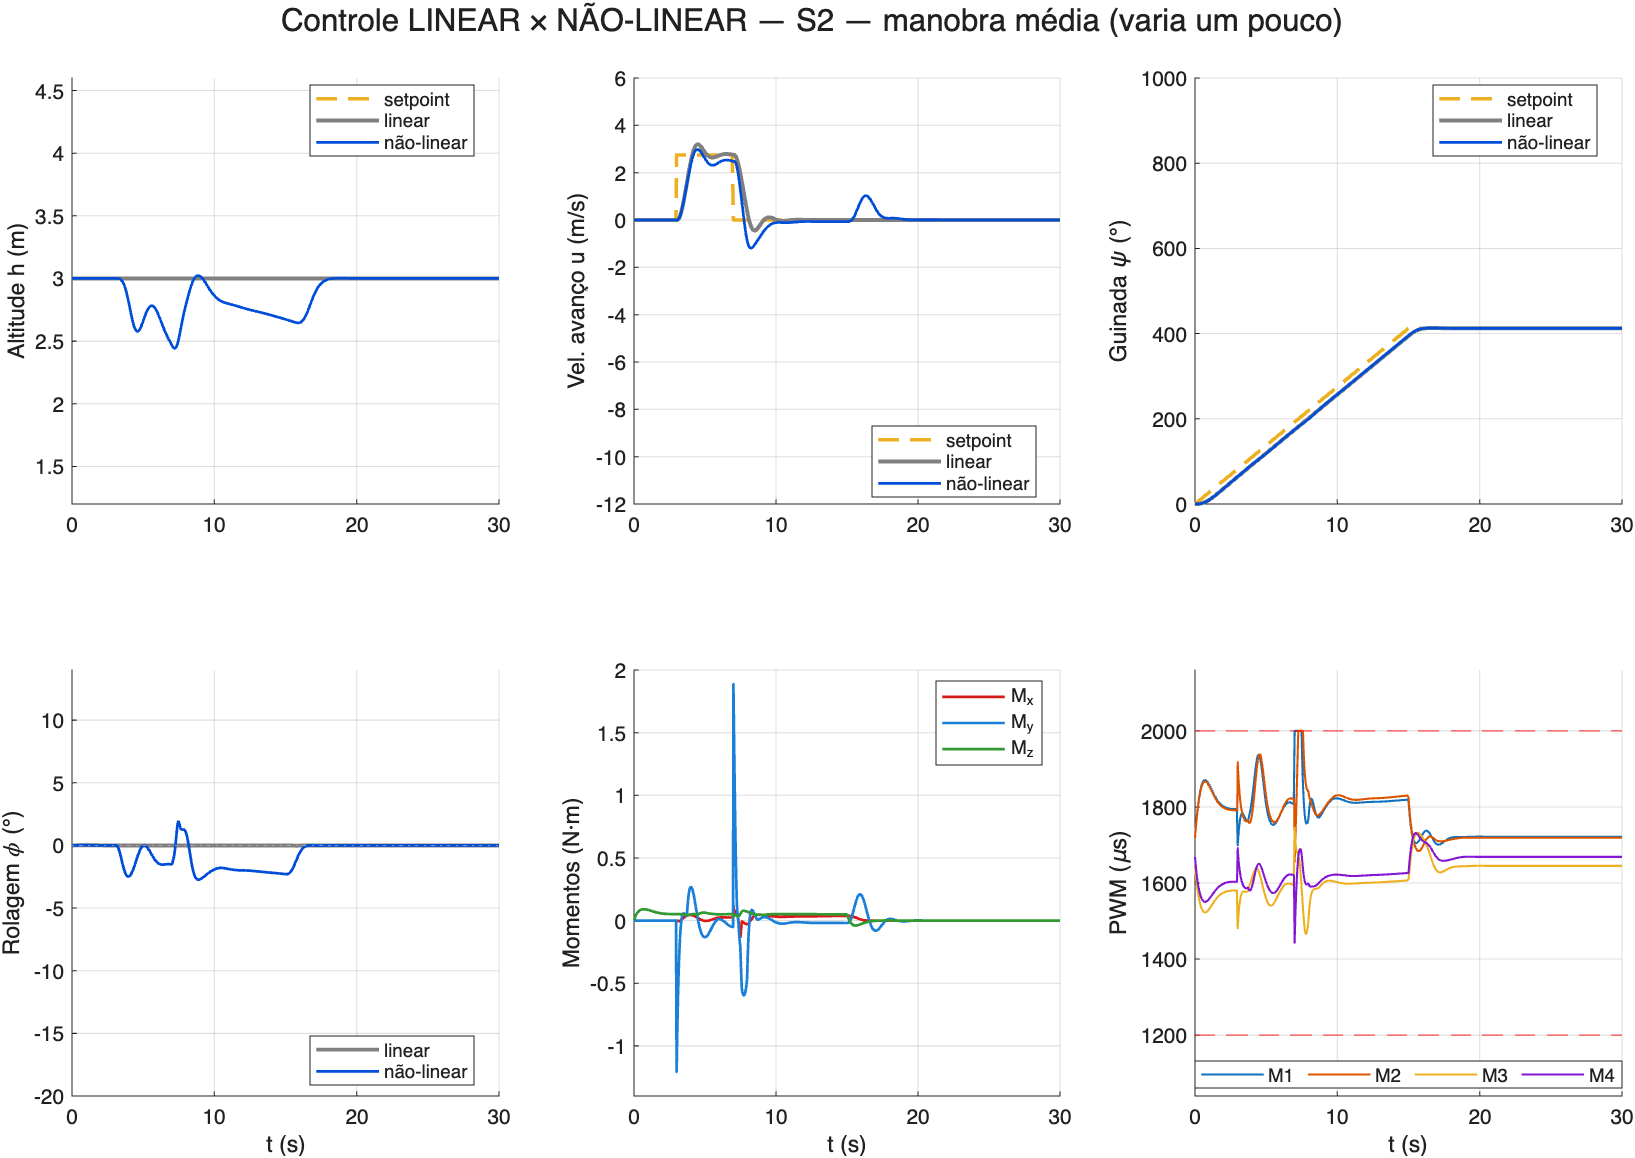
\includegraphics[width=\textwidth]{Cap5/sim_ctrl_s2_pouco.png}
    \caption{Cenário $S_2$ (manobra média): a altitude do não linear afunda e surge rolagem por acoplamento giroscópico, ausente no linear{\color{blue}. Durante o giro, ambas mantêm desvio sustentado de pequena amplitude, e convergem às referências quando ele cessa, em $15$~s}.}
    \label{fig:ctrl-s2}
\end{figure}

No cenário forte $S_3$ (Figura~\ref{fig:ctrl-s3}), as duas previsões descolam por completo. O modelo linear prevê uma resposta benigna, altitude nivelada, rolagem nula, mas, na planta real, {\color{blue}a inclinação do empuxo faz a altitude afundar cerca de $1{,}4$\,m (de $3$ para $1{,}6$\,m) e em seguida ultrapassar a referência em até $1{,}6$\,m, o acoplamento giroscópico leva a rolagem a $-11^\circ$ e a velocidade de avanço diverge da referência em mais de $9$\,m/s. Esse cenário opera no limite de autoridade do controlador na planta não linear: sob a guinada sustentada de $45^\circ$/s combinada com a arfagem, o controlador projetado no modelo desacoplado deixa de regular a rolagem e o avanço, ainda que a resposta permaneça limitada enquanto o giro dura. Encerrado o giro, em $15$~s, o acoplamento que sustentava os desvios desaparece e a aeronave converge ao voo pairado em poucos segundos, recuperando altitude, rolagem e avanço, comportamento que o próprio modelo linear, por construção, não consegue prever, já que para ele a manobra nem sequer perturba esses canais.}

\begin{figure}[H]
    \centering
    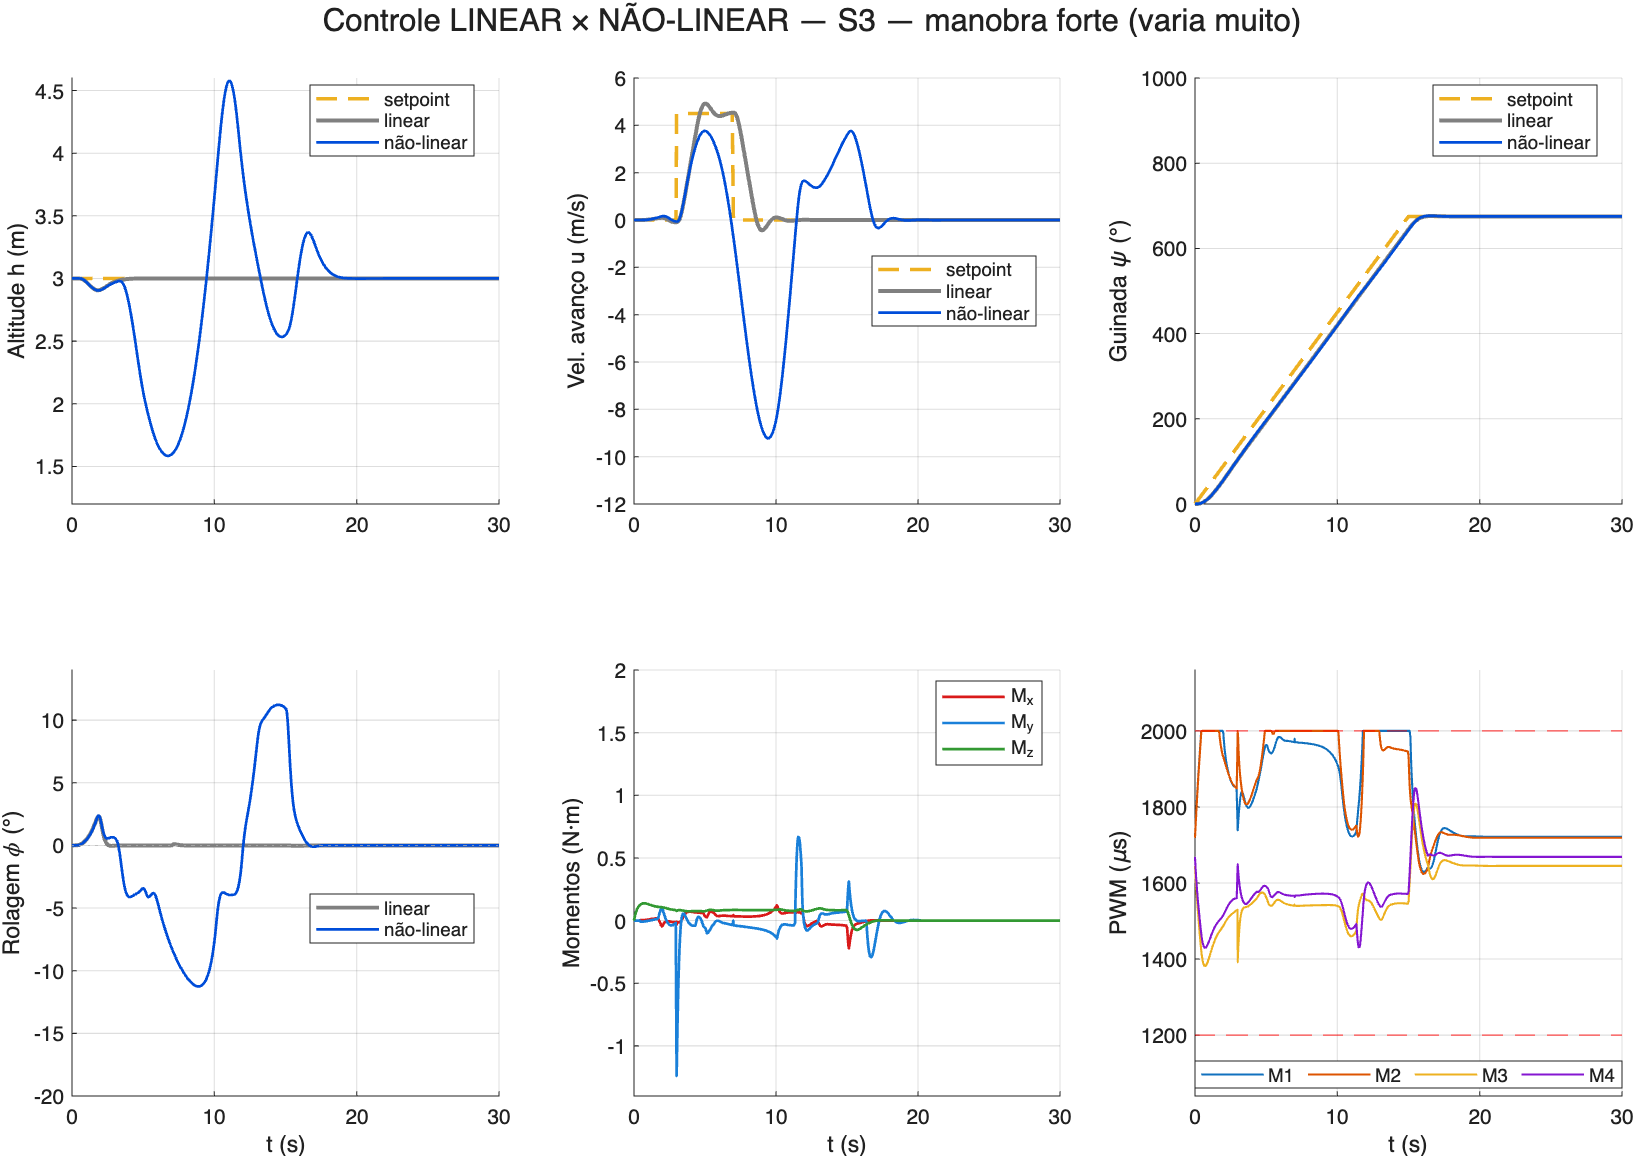
\includegraphics[width=\textwidth]{Cap5/sim_ctrl_s3_muito.png}
    \caption{\color{blue}Cenário $S_3$ (manobra forte): as plantas descolam, o não linear afunda cerca de $1{,}4$\,m em altitude e atinge $-11^\circ$ de rolagem, enquanto o linear prevê resposta estável. Após o fim do giro, em $15$~s, o não linear converge ao voo pairado.}
    \label{fig:ctrl-s3}
\end{figure}

Em conjunto, os três cenários delimitam a faixa de validade do modelo linear para fins de controle: excelente para manobras dentro do envelope de voo pairado ($S_1$), adequado com ressalvas para manobras moderadas ($S_2$), em que os acoplamentos já produzem desvios {\color{blue}de altitude e rolagem sustentados enquanto a manobra dura} e inadequado para manobras agressivas e acopladas ($S_3$), nas quais os termos giroscópicos e a inclinação do empuxo, desprezados na linearização, dominam a resposta. O resultado justifica o uso do modelo não linear identificado como banco de provas do controlador em simulação. Cabe reiterar que o controlador aqui projetado não foi embarcado nem ensaiado em voo, conforme o escopo definido no Capítulo~1: a validação experimental do trabalho concentra-se no modelo, confrontado com dados reais de voo, ao passo que o controle é avaliado exclusivamente sobre esse modelo validado. O ensaio em voo do controlador constitui a etapa natural seguinte, discutida no Capítulo~6.
